\documentclass[12pt,a4paper,headsepline,footsepline,DIV13,BCOR12mm]{scrbook}
\usepackage[english,ngerman]{babel}
\usepackage[T1]{fontenc}
\usepackage[latin1]{inputenc}
\usepackage{scrpage2}
\pagestyle{scrheadings}
\usepackage{setspace}
\usepackage[font=singlespacing]{caption}
\usepackage{graphicx}
\usepackage{subfigure}
\usepackage{listings}
\usepackage{comment}

\lstset{ % default settings for listings from http://en.wikibooks.org/wiki/LaTeX/Packages/Listings
  captionpos=b,                   % sets the caption-position to bottom
  breaklines=true                % sets automatic line breaking
}

%create pdf hyperlinks with a color box (will not be printed)
\usepackage{hyperref}
\hypersetup{colorlinks=false}

% todo and review commands
\usepackage{soul}
\usepackage{color}
%\newcommand{\hl}[1]{\fcolorbox{red}{white}{#1}} %fcolorbox does not break lines properly
\newcommand{\todo}[1]{{\color{red}{\hl{TODO: #1...}}}}
\newcommand{\review}[0]{\todo{REVIEW}}
\newcommand{\comm}[1]{\textsuperscript{\bf \color{red}{\tiny [#1]}}}
\newcommand{\q}[0]{\comm{?}}
\newcommand{\s}[0]{\comm{*}}


\begin{document}

% begin preface
\selectlanguage{ngerman}
%%%%%%%%%%%%%%%%%%%%%%%%%%%%%%%%%%%%%%%%%%%%%%%%%%%%%%%%%%%%%%%%%%%%%%%%%%%%%%%%%%%%
%%% Title-Page
\thispagestyle{empty}

\begin{table}[h]
\centering
\begin{tabular}{ccc}

\includegraphics[width=.18\linewidth]{img/logos/lmu_logo} \hspace{0.7cm} &

\includegraphics[scale=0.18]{img/logos/Uni_Aug_Logo_Basis_pos_A}
\hspace{0.7cm} &

\includegraphics[scale=0.86]{img/logos/tum}
\end{tabular}
\end{table}

\vspace{8mm}
\begin{center}
{\Large
{\bfseries \scshape Institut f�r Software \& Systems Engineering}\\
Universit�tsstra�e 6a \hspace{0.25cm} D-86135 Augsburg\\
}
\end{center}

\vspace{1cm}
%title
\begin{center}
{\Huge \bfseries A flexible visual framework  \\
\vspace{0.25cm}
for debugging complex robotic systems}
\end{center}

\vspace{1.5cm}
%author
\begin{center}
{\Large Felix Kaser}
\end{center}

\vspace{1cm}
\begin{center}
{\Large \bfseries Masterarbeit im Elitestudiengang Software Engineering}
\end{center}

\vspace{1cm}
\begin{center}

\includegraphics[width=.4\linewidth]{img/logos/LogoSEengl}
\end{center}



%%%%%%%%%%%%%%%%%%%%%%%%%%%%%%%%%%%%%%%%%%%%%%%%%%%%%%%%%%%%%%%%%%%%%%%%%%%%%%%%%%%%
%%% Advisor-Page
%%%%%%%%%%%%%%%%%%%%%%%%%%%%%%%%%%%%%%%%%%%%%%%%%%%%%%%%%%%%%%%%%%%%%%%%%%%%%%%%%%%%
\newpage
\thispagestyle{empty}
\mbox{}
\newpage
\thispagestyle{empty}

\begin{table}[h]
\centering
\begin{tabular}{ccc}

\includegraphics[width=.18\linewidth]{img/logos/lmu_logo} \hspace{0.7cm} &

\includegraphics[scale=0.18]{img/logos/Uni_Aug_Logo_Basis_pos_A}
\hspace{0.7cm} &

\includegraphics[scale=0.86]{img/logos/tum}
\end{tabular}
\end{table}

\vspace{1cm}
\begin{center}
{\Large
{\bfseries \scshape Institut f�r Software \& Systems Engineering}\\
Universit�tsstra�e 6a \hspace{0.25cm} D-86135 Augsburg\\
}
\end{center}

\vspace{2cm}
%title
\begin{center}
{\Huge \bfseries A flexible visual framework  \\
\vspace{0.25cm}
for debugging complex robotic systems}
\end{center}

\vspace{0.7cm}
%author
\begin{center}
\begin{table}[h]
\centering
\begin{tabular}{ll}
Matrikelnummer: & 1174068 \\
Beginn der Arbeit: & 21.\ Juni 2012 \\ 
Abgabe der Arbeit: & XX.\ XXXX 2012 \comm{datum} \\
Erstgutachter: & Prof.\ Dr.\ Wolfgang Reif \\
Zweitgutachter: & Prof.\ Dr.\ Bernhard Bauer \\
Betreuer: & M.Sc. Andreas Angerer \comm{\& bruce?} \\
\end{tabular}
\end{table}
\end{center}

\vspace{0.25cm}
\begin{center}

\includegraphics[width=.4\linewidth]{img/logos/LogoSEengl}
\end{center}

%%%%%%%%%%%%%%%%%%%%%%%%%%%%%%%%%%%%%%%%%%%%%%%%%%%%%%%%%%%%%%%%%%%%%%%%%%%%%%%%%%%%
%%% Statement-Page
\newpage
\thispagestyle{empty}
\mbox{}
\newpage
\thispagestyle{empty}

\centerline{\bfseries ERKL�RUNG}

\vspace{5cm}
Hiermit versichere ich, dass ich diese Masterarbeit selbst�ndig verfasst habe.
Ich habe dazu keine anderen als die angegebenen Quellen und Hilfsmittel
verwendet.

\vspace{1cm}
\begin{flushleft}
%select german for formatting the date
\selectlanguage{ngerman}
Augsburg, den \todo{datum} \hfill Felix Kaser
\end{flushleft}

\newpage
\thispagestyle{empty}
\mbox{}

 
\newpage

\renewcommand{\baselinestretch}{2} % zeilenabstand

%select english as language!
\selectlanguage{english}

\pagenumbering{roman}
\chapter*{Acknowledgements}
I would like to thank everyone who supported me in the last months either by providing professional advice and guidance or just being a good friend and listen to my ideas and thoughts. This work would have never been possible without the support from Prof. Dr. Wolfang Reif, who established the connection to the University of Auckland in New Zealand, Dr. Dominik Haneberg, who made the exchange possible and Andreas Angerer who helped me to find my way and write this thesis. I would also like to thank the Robotics Group at the University of Auckland under the supervision of Assoc. Prof. Bruce MacDonald, where I was able to work on the project. You inspired me with the work you do and were of great help whenever I needed it.

No words can express how thankful I am for the support of my parents Annemarie and Martin, and my sister Lisa. Thank you for your never ending support. I can count on you in good times and in bad.

There are so many people who helped me, it is hard to name them all. I thank you, if you ever had a coffee with me and talked with me about work and the life beyond work.

\newpage
\chapter*{Abstract}
Data collected during debugging is traditionally rendered as text. The special application field of robotics faces problems with this approach, since a typical robotic system constantly gathers and processes data from the surrounding environment through sensors. Robotic applications are also hard to interrupt during debugging, since robots generally don't run in a deterministic and suspendable environment. Developers of robotic applications are confronted with high amounts of data during debugging, which becomes hard to interpret if the data is represented as text and high amounts of data need to be interpreted at once.

This thesis tries to solve this problem by introducing a visual debugging system to support debugging of robotic applications: It takes into account the special requirements for a debugging tool in a robotic development environment, especially the uninterrupted rendering of debugging data and the need for better visualization of data to support a faster interpretation of data. The goal of the developed system is to help developers understand the data during debugging more quickly and improve overall productivity during robot development. To achieve the goal a system was designed and developed where developers can choose how they want to visualize data collected during debugging of a robotic application. This work presents the system design and a prototypical implementation of the proposed system. Evaluating the hypothesis that the developed system can improve productivity during debugging is out of scope for this work but initial experiments were promising and the developed tool provides a solid base for further evaluations.
\newpage
\chapter*{TODOS}
\todo{listing positions}\\
\todo{dates on title pages}\\
\todo{general layout}\\
\newpage
\tableofcontents
\newpage
\listoffigures
\newpage
%\listoftables
\lstlistoflistings

\pagenumbering{arabic}
%end preface

\chapter{Introduction}

This will become the glorious introduction section. Make sure to write it in
the end and not in the beginning.

\section{Problem Statement}
\label{problem_statement}
[\textbf{problems with robotic software, many different environments, not interruptable, ...}]
Debugging robotic systems can prove to be much more complicated then normal software systems. 

\section{ROS}
The Robot Operating System (ROS) is an Open Source framework for complex robotic systems. The first work on ROS was done as part of the STanford Artificial Intelligence Robot (STAIR) in 2007 \cite{Quigley2007}. The original software library was called \emph{Switchyard} and had been developed at Stanford. Later the library was refined and generalized to also suit the requirements of the Personal Robot Program at Willow Garage\footnote{www.willowgarage.com} \cite{Quigley2009}. The resulting general framework has been released as Open Source \cite{Quigley2009} and this section gives a short overview over the most important principles in ROS.

\begin{figure}[ht]
\centering
\subfigure[Stanford's STAIR]{
	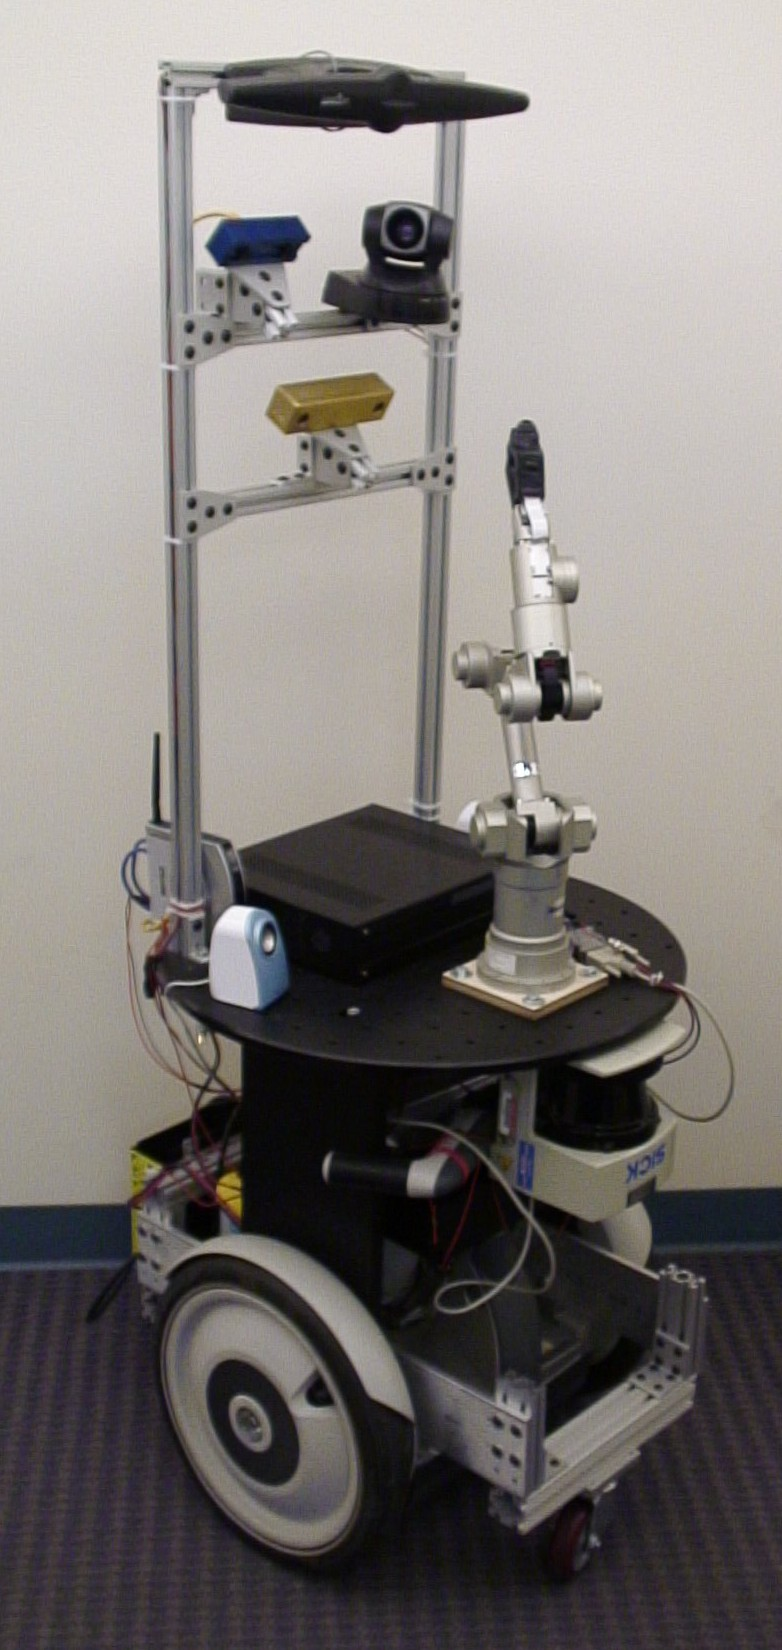
\includegraphics[height=8cm]{img/stair}
}
\subfigure[Willow Garage's PR2]{
	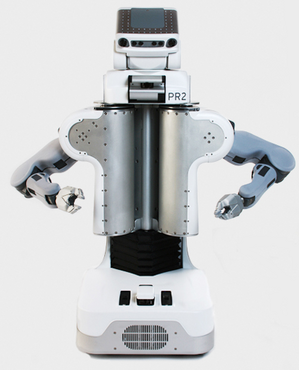
\includegraphics[height=8cm]{img/pr2}
}
\end{figure}

ROS was built to abstract from the hardware of the robot and create modular robot software, which can run on different robots and on different machines. This makes it easier to write software for robots and distribute the work to different teams, each team focusing on one part of the robot. The modules in ROS are called nodes and several nodes executed together are called a stack. ROS packages bundle nodes and stacks and are used to make software modules available to other developers. Everyone can create their own package which can be indexed by ROS so that your software modules can be found, downloaded and used by other developers. There exist many packages, nodes and stacks for some of the most common problems in robotics (e.g. navigation, localization, joint movement, etc.) and can easily be re-used.

The communication between ROS nodes can be done asynchronously through a publish/subscribe mechanism and synchronously through services. Nodes can send messages by publishing a message on a topic and receive messages by subscribing to that topic. This mechanism is really flexible and decouples the sender from the receiver. A publisher node does not need to know if there are other nodes listening and vice versa. For synchronous communication and guaranteed delivery of messages, services can be invoked. The routing is established during runtime through the ROS core. The core of ROS was kept really slim and only contains the most essential parts of the framework (such as the inter node communication). ROS can run on several machines distributed in a network, the only restriction is that every node needs to know the address of the core (master node) in order to communicate with other nodes.

[\textbf{review this paragraph}]

A variety of tools have been built around the ROS core to facilitate the development of ROS nodes and robotic software in general. They help you to create packages, nodes and stacks and execute and debug them. The philosophy for those tools is to be small and do one job only but do it good. This results in a really robust tools similar to the toolchain available on Linux. The downside is a big variety of tools in the ROS ecosystem, which can be confusing to new developers. See \ref{related_ros_tools} for a more detailed analysis of current ROS tools.

The latest stable version of the ROS framework was released in April 2012 (ROS Fuerte). Previous releases of stable versions have been in August 2011 (ROS Electric), March 2011 (ROS Diamondback), August 2010 (ROS C Turtle) and March 2010 (ROS Box Turtle). There are currently many institutions, companies and individuals involved in the ROS community, contributing in many different ways. This makes ROS a god target platform, since we want to reach as many developers as possible (see \ref{availability_developers}).

\section{Visualization}
This is problably too much literature review to go through...

\section{Outline}
Explain all the chapters and sections of this work.

\chapter{Related Work}

\section{ROS}
The Robot Operating System (ROS) is an Open Source framework for complex robotic systems. The first work on ROS was done as part of the STanford Artificial Intelligence Robot (STAIR) in 2007 \cite{Quigley2007}. The original software library was called \emph{Switchyard} and had been developed at Stanford. Later the library was refined and generalized to also suit the requirements of the Personal Robot Program at Willow Garage\footnote{www.willowgarage.com} \cite{Quigley2009}. The resulting general framework has been released as Open Source \cite{Quigley2009} and this section gives a short overview over the most important principles in ROS.

\begin{figure}[ht]
\centering
\subfigure[Stanford's STAIR]{
	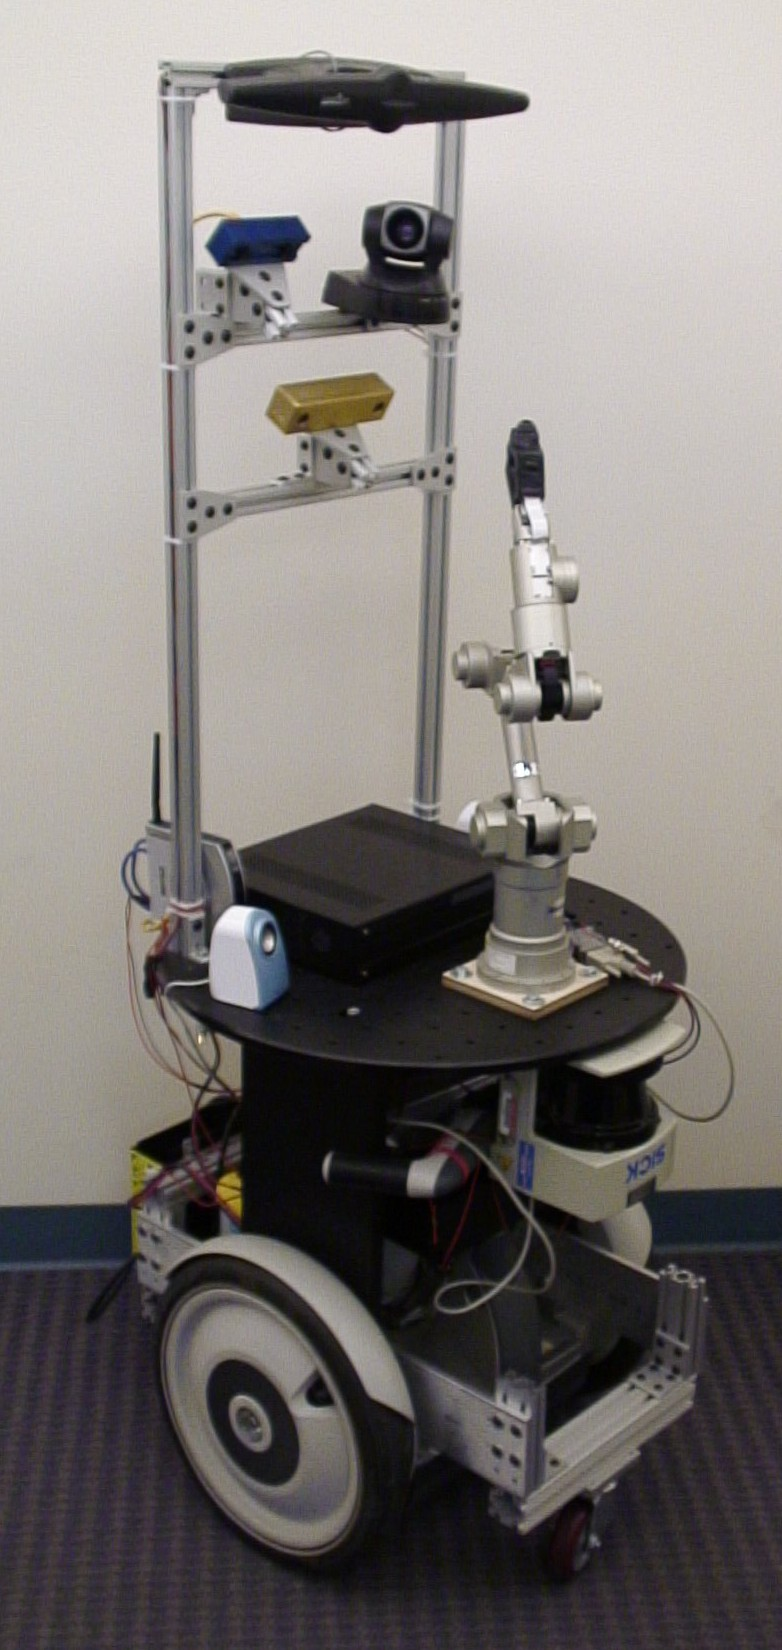
\includegraphics[height=8cm]{img/stair}
}
\subfigure[Willow Garage's PR2]{
	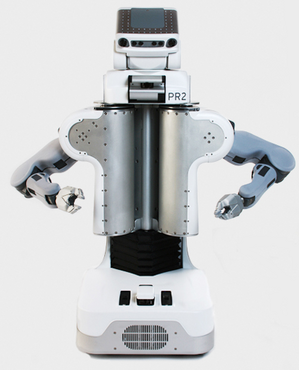
\includegraphics[height=8cm]{img/pr2}
}
\end{figure}

ROS was built to abstract from the hardware of the robot and create modular robot software, which can run on different robots and on different machines. This makes it easier to write software for robots and distribute the work to different teams, each team focusing on one part of the robot. The modules in ROS are called nodes and several nodes executed together are called a stack. ROS packages bundle nodes and stacks and are used to make software modules available to other developers. Everyone can create their own package which can be indexed by ROS so that your software modules can be found, downloaded and used by other developers. There exist many packages, nodes and stacks for some of the most common problems in robotics (e.g. navigation, localization, joint movement, etc.) and can easily be re-used.

The communication between ROS nodes can be done asynchronously through a publish/subscribe mechanism and synchronously through services. Nodes can send messages by publishing a message on a topic and receive messages by subscribing to that topic. This mechanism is really flexible and decouples the sender from the receiver. A publisher node does not need to know if there are other nodes listening and vice versa. For synchronous communication and guaranteed delivery of messages, services can be invoked. The routing is established during runtime through the ROS core. The core of ROS was kept really slim and only contains the most essential parts of the framework (such as the inter node communication). ROS can run on several machines distributed in a network, the only restriction is that every node needs to know the address of the core (master node) in order to communicate with other nodes.

[\textbf{review this paragraph}]

A variety of tools have been built around the ROS core to facilitate the development of ROS nodes and robotic software in general. They help you to create packages, nodes and stacks and execute and debug them. The philosophy for those tools is to be small and do one job only but do it good. This results in a really robust tools similar to the toolchain available on Linux. The downside is a big variety of tools in the ROS ecosystem, which can be confusing to new developers.

The latest stable version of the ROS framework was released in April 2012 (ROS Fuerte). Previous releases of stable versions have been in August 2011 (ROS Electric), March 2011 (ROS Diamondback), August 2010 (ROS C Turtle) and March 2010 (ROS Box Turtle). There are currently many institutions, companies and individuals involved in the ROS community, contributing in many different ways.

[\textbf{make a reference to the requirements: availability to developers}]
\section{Tracepoints}
[\textbf{Luke Gumbleys work, tracepoint theory, adaptation in robotics, instrumentation}]
\cite{Gumbley2009}

\section{rxDeveloper}
[\textbf{outline, results of the survey, importance for this work}]
\cite{Muellers2012}

\section{Other Debugging Work}
[\textbf{android logging?, ROS logging?, AR debugging?}]



\chapter{Design of a Flexible Visual Debugging System}
\label{visual_debugging_system}

Debugging in robotics has unique requirements which are often not met by traditional debugging systems. The special requirements lead to a number of different tools to support debugging in robotics. The previous chapter summarized some of those tools and issues of existing solutions were identified: a) The tools either focus on visualization of pre-defined spatial data or render data as text messages. b) The graphical interfaces are rather static and difficult to adapt to different usage scenarios.

This chapter introduces a new system for debugging in robotics, tailored to tackle the challanges developers face when debugging robotic systems. The system tries to combine the ease of use and flexibility of logging statements with a graphical visualization. The visualization makes it easier to comprehend the high amount of data collected during debugging of robotic systems.

The first section states the hypothesis behind the ideas that have driven the development of the debugging system. Section two presents the goals of the work, which leads to specific requirements for this system in section three. The system design section presents the design for a flexible visual debugging system.

%Write about the general requirements for a visual debugging system, rosdashboard would be one possible implementation. This basically could explain most of rosdashboard, apart from the ros specific part which is: topic subscription setup (gui), topic introspection to wait for message class types, topic subscription (code) and calling the value update hook. Saving to file saves the topic configuration which is ros specific as well.

%Point out that ROS was targeted early on and affected many decisions, but the requirements and the system design is applicable in general. [Andreas: not sure if this is the right place, might be better in the introduction, since it explains the dominance of ROS tools in related work / debugging in robotics]

%--> Generalize design decisions, if they apply for other robot frameworks as well.

%%%% HYPOTHESIS %%%%
\section{Hypothesis}
A possible reason why many developers still use print or logging statements to debug their programs is because these methods can be immediately used when required. Developers don't need to undergo a lengthy setup and configuration process before they can start debugging and they don't need to gain extensive knowledge about the methodology and tools either. The overhead to set up and configure a debugging system should be reduced to make the system easy to use without extensive knowledge about the debugging methodology and tool.

The main issue with print or logging statements is the text-only representation of data. The system proposed in this chapter aims to support the developer during debugging by visualizing data in a graphic way and thus eliminate the cognitive effort needed to parse and interpret text based logging messages. The cognitive effort required during debugging can be further reduced by a flexible system which can be adapted to different preferences of different developers. Every developer can choose a visualization that fits their mental model of the debugged data best.


%%%% GOALS %%%%
\section{Goals}
The main goal of this work is to design a debugging system which is suitable for debugging in robotics and can be used to evaluate the hypothesis stated above. The design of the system is independent of a specific robotic framework and could be implemented for any available framework.
While most of the currently available visualization tools in robotics focus on pre-defined and spatial data to help understand the robot and the environment in which it runs \cite{Collett2010, Quigley2009}, rendering of abstract data is still uncommon. The design of the debugging system should be flexible enough to allow visualization of arbitrary and abstract data. Although abstract data will be the main focus of the debugging system since tools to visualize pre-defined data are already widely available, the designed system is not restricted to abstract data.

The system provides a graphical user interface which can be used by developers to visualize all kinds of data from the robotic application. The developers can customize the visualization according to the current robot hardware, development stage and personal preferences. The system can be adapted to many different use cases and should reduce the cognitive effort during debugging by visualizing the data according to the mental model of the developer and meaning of the data.

\todo{where to put the save and restore functionality? it is shown in the object model and could be a possible requirements: saving and loading dashboards allows to distribute the dashboard amongst developers, all the configuration is stored within the dashboard file. Maybe goals, maybe requirements, maybe user interface}

%%%% REQUIREMENTS %%%%
\section{Requirements}
\label{requirements}
The requirements of the flexible visual debugging system are mostly dominated by the special requirements of robotics. Some requirements are derived from the hypothesis and focus more on development performance and speed. This section presents the elicited requirements for a flexible visual debugging system.

\subsection{Distributed Live Debugging}
When debugging robotic applications it is usually not possible to interrupt the execution of the application and follow a step-through approach. All data must be captured, processed and visualized live. Robotic applications are usually distributed systems, because they often run on mobile robots or are so complex that multiple computers are used to make the system faster. This means the system must be able to handle communication distributed across a network.

\subsection{Adaptable Tool}
Due to many different application scenarios in robotics and the diverse environment of available frameworks for robot development, many researchers and developers have built their own tools to support them during debugging \cite{Collett2010}. Developing your own debugging tool is extremely time consuming and the developed tools are often one-time-only tools, because they don't fit the use case of other applications and are too hard to adapt to a new project.
In order to allow the use of the proposed debugging system in many different scenarios and use cases, flexibility has a high priority. Flexibility not only means the system can be adapted easily to fit different problems, it also means the system can be adapted to suit different developer's preferences. Each developer might prefer a different kind of visualization of the collected data, thus loose coupling of the collected data and the visualization widgets is necessary.

\subsection{Low Configuration Overhead}
Debugging robotic applications is a highly iterative process, where small changes are made and immediately deployed to the robot. When the new visualizations are needed or old visualizations need to be updated, the configuration overhead should be as minimal as possible so that the developer is not distracted from the problem analysis task. The configuration task should not distract the developer from the problem analysis task.

%%%% SYSTEM DESIGN %%%%
\section{System Design}
\label{system_design_section}
The design of the developed system reflects the requirements identified in Section~\ref{requirements}. The system is designed to run in a distributed environment and visualize data live, as it is collected and not post-mortem. The system design is not tailored to a specific robotic framework: Since the underlying communication architecture is similar in most robotic systems, implementing the system for any robotic system is possible.
Although the design is robot framework unspecific, it was influenced by the ROS architecture since the documentation of ROS is good and the community was helpful when questions arose. \q
The need for an adaptable system influenced especially the object design, which takes into consideration the future extendibility and adaptability during the debugging process.

This section shows how the system is designed according to the requirements: The user interface design, the system architecture and the object design are presented. The user interface is presented first, because the concept of a developer dashboard influenced both the architecture and the object design.

\subsection{Graphical User Interface}
\label{graphical_user_interface}
In order to be adaptable to many different use cases and visualization preferences of developers, a central dashboard approach was chosen for the user interface. The dashboard allows developers to add and remove visualizations easily and arrange them however they want. The visualizations are wrapped in widgets and can thus be positioned freely on the dashboard. Adding new visualizations to the dashboard can be done through a "Drag \& Drop" mechanism, once the widget is on the dashboard it can be resized and repositioned on the canvas. The initial mockup of the proposed graphical user interface is shown in Figure~\ref{gui_mockup}.

\begin{figure}[htbp]
  \centering
  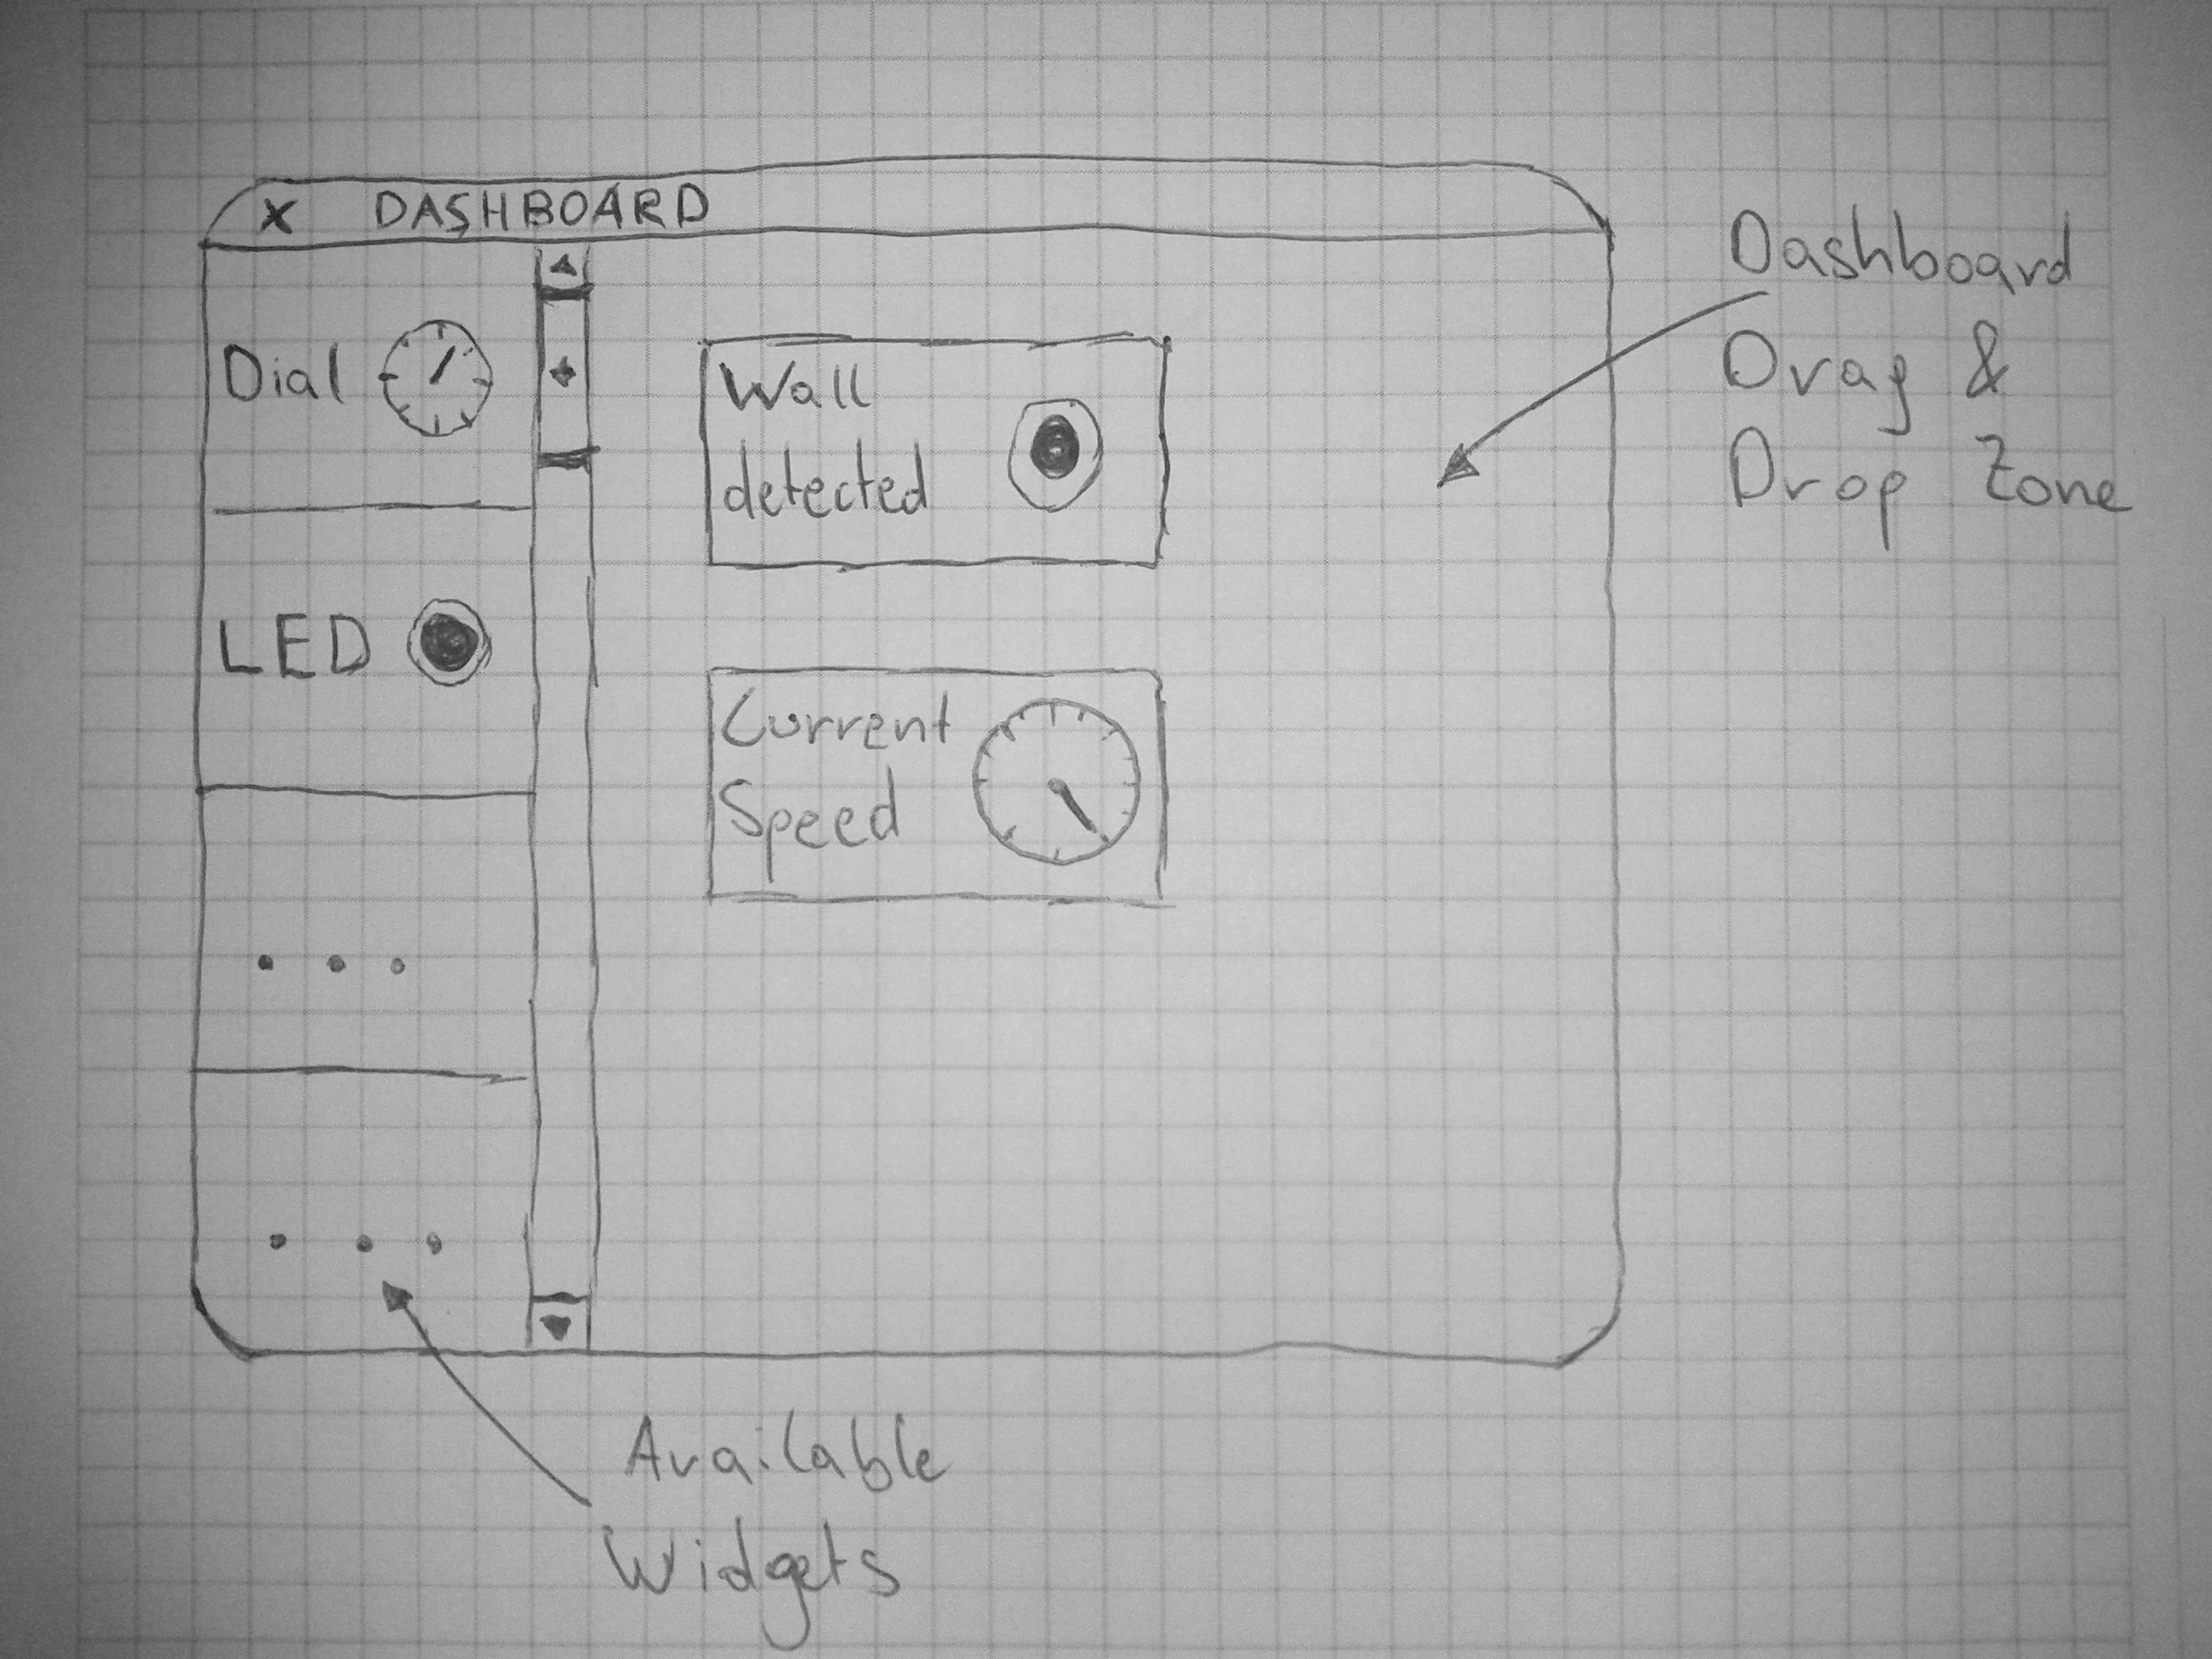
\includegraphics[width=\textwidth]{img/initial_gui_mockup.jpg}
  \caption{Paper mockup for the graphical interface.}
  \label{gui_mockup}
\end{figure}

Each item in the list on the left (Figure~\ref{gui_mockup}) represents one type of visualization, this can be as simple as a dial for numeric values or more complex visualizations for more concrete data like a map visualization. Although the design of the user interface does not restrict the types of visualizations, it is intended for simple and abstract data, since other tools like RViz (see Section~\ref{rviz}) are more specialized for complex and spatial data required in other use cases.

\begin{figure}[htbp]
  \centering
  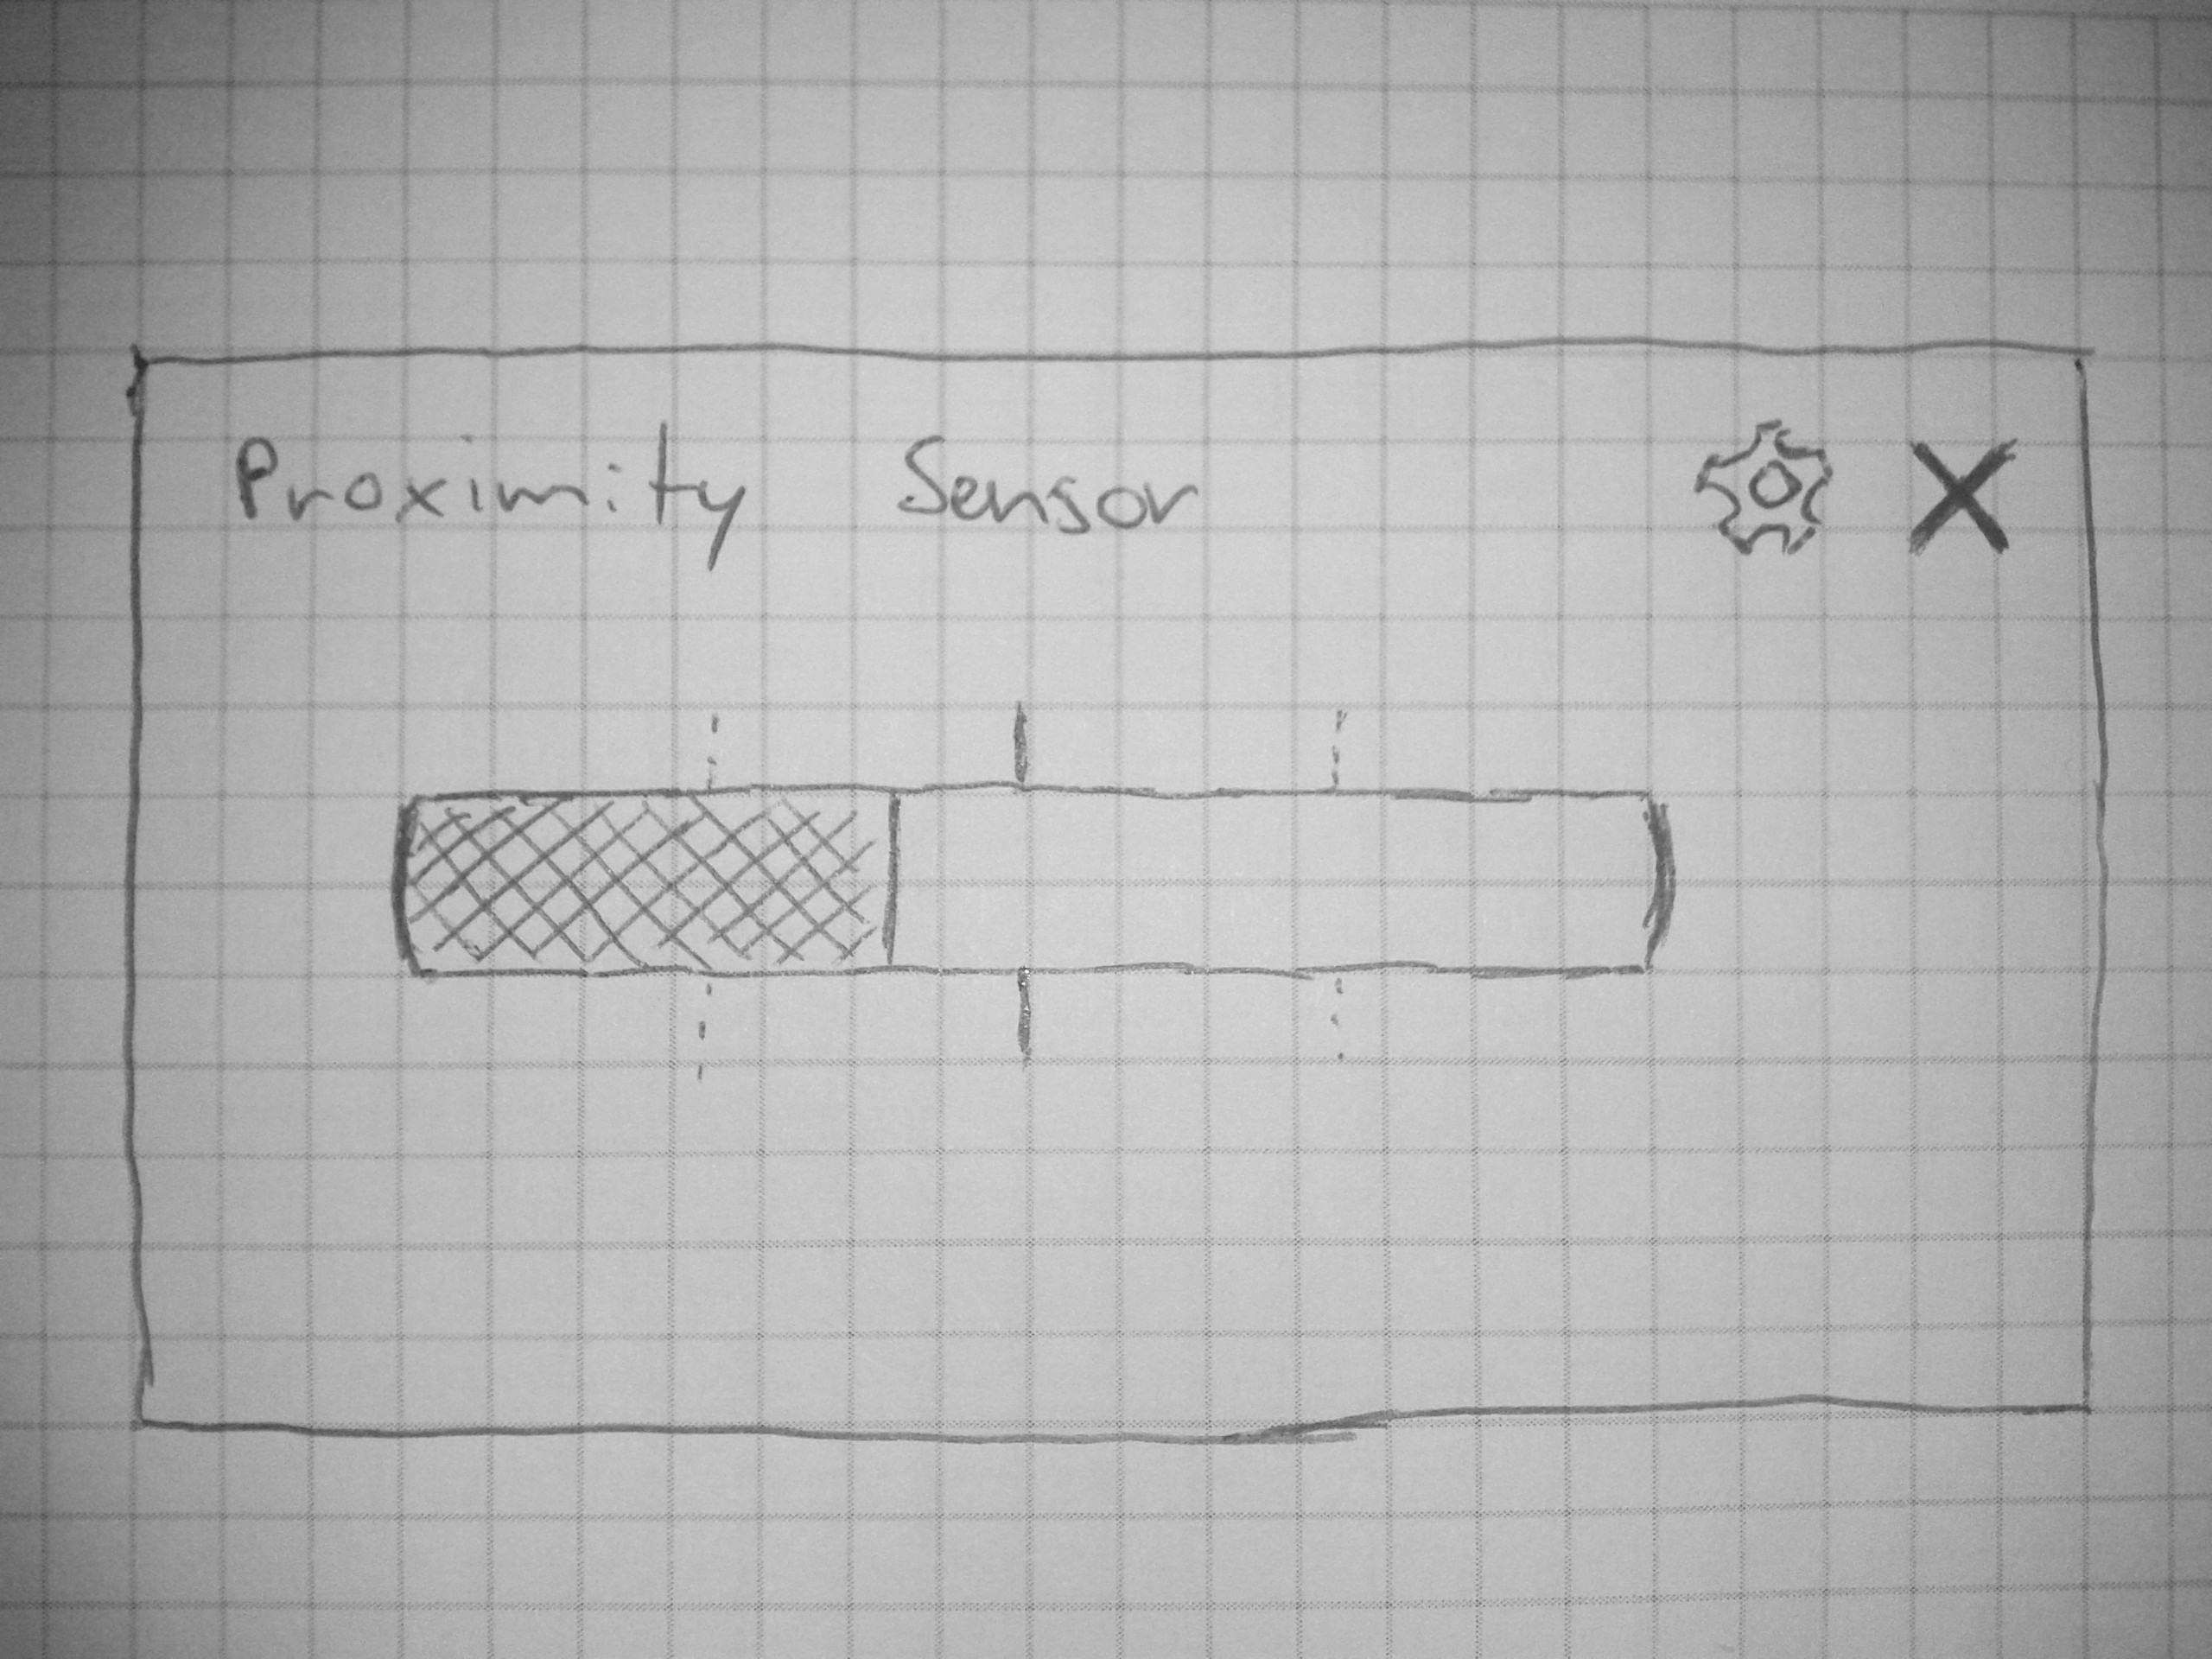
\includegraphics[width=.5\textwidth]{img/initial_widget_mockup.jpg}
  \caption{Paper mockup for a visualization widget.}
  \label{widget_mockup}
\end{figure}

Figure~\ref{widget_mockup} shows an early mockup of a visualzation widget on the dashboard. This exemplary visualization widget has the form of a progress bar where numeric values can be visualized. Dials, meters, thresholds, compasses and LEDs could be other simple visualizations widgets. A more complex example for a visualization widget is the laser scan visualization as shown in Figure~7 in Luke Gumbley's paper on realtime debugging \cite{Gumbley2009}.
\comm{Should I copy the screenshot from \cite{Gumbley2009} or only cite it?}
%The widgets can be hooked up to data providers and will be updated once a new value is available.

\todo{Write about the communication setup here, since it is referenced in the architecture. ---> imho this is too implementation specific and should be left out: rewrite the architecture part to be more general}

\subsection{Architecture}
The currently available robotic frameworks all rely on a communication middleware that abstracts from the concrete communication channels. This communication infrastructure can be used by the proposed debugging system to access data without the need to develop a dedicated communication layer for debugging.

The user interface mockup shown in Figure~\ref{gui_mockup} already indicates the modular design of visualizations that can be added to the dashboard canvas. The modular approach makes it easy to extend the system with more visualizations in the future and it gives developers the choice how data is visualized. Each visualization widget contains a different form of visualization. This visualization widget handles the graphical part of the visualization, stores information about the data connection and other settings and encapsulates the communication with the middleware. The connection with the communication middleware is established through an adapter which notifies the widget if the data has changed or new data is available. This makes it easy to exchange the communication adapter if the communication protocol changes or the implementation targets a different robotic framework which has a different communication structure. This reduces the coupling between the visualizations and the data collection. Although the dashboard needs to know which widgets are currently on the dashboard, the widgets itself are independent of the dashboard. The decentralized approach allows easier integration of a plugin infrastructure since the dashboard itself does not need to be modified to show additional visualization widgets.

Figure~\ref{communication_diagram} shows how the modular visualization widgets connect to the communication middleware through the adapter. The robot modules at the bottom of the diagram publish data of some kind: either data which is needed to communicate with other modules or data specifically emitted for debugging. The visualizations can connect to both kinds of data through the middleware.

\q In order to tell the visualizations what data they should visualize, a graphical interface for setting up the communication details has been presented in \ref{graphical_user_interface}. \q
\todo{make the above more general or drop completely}

\begin{figure}%[htbp]
  \centering
  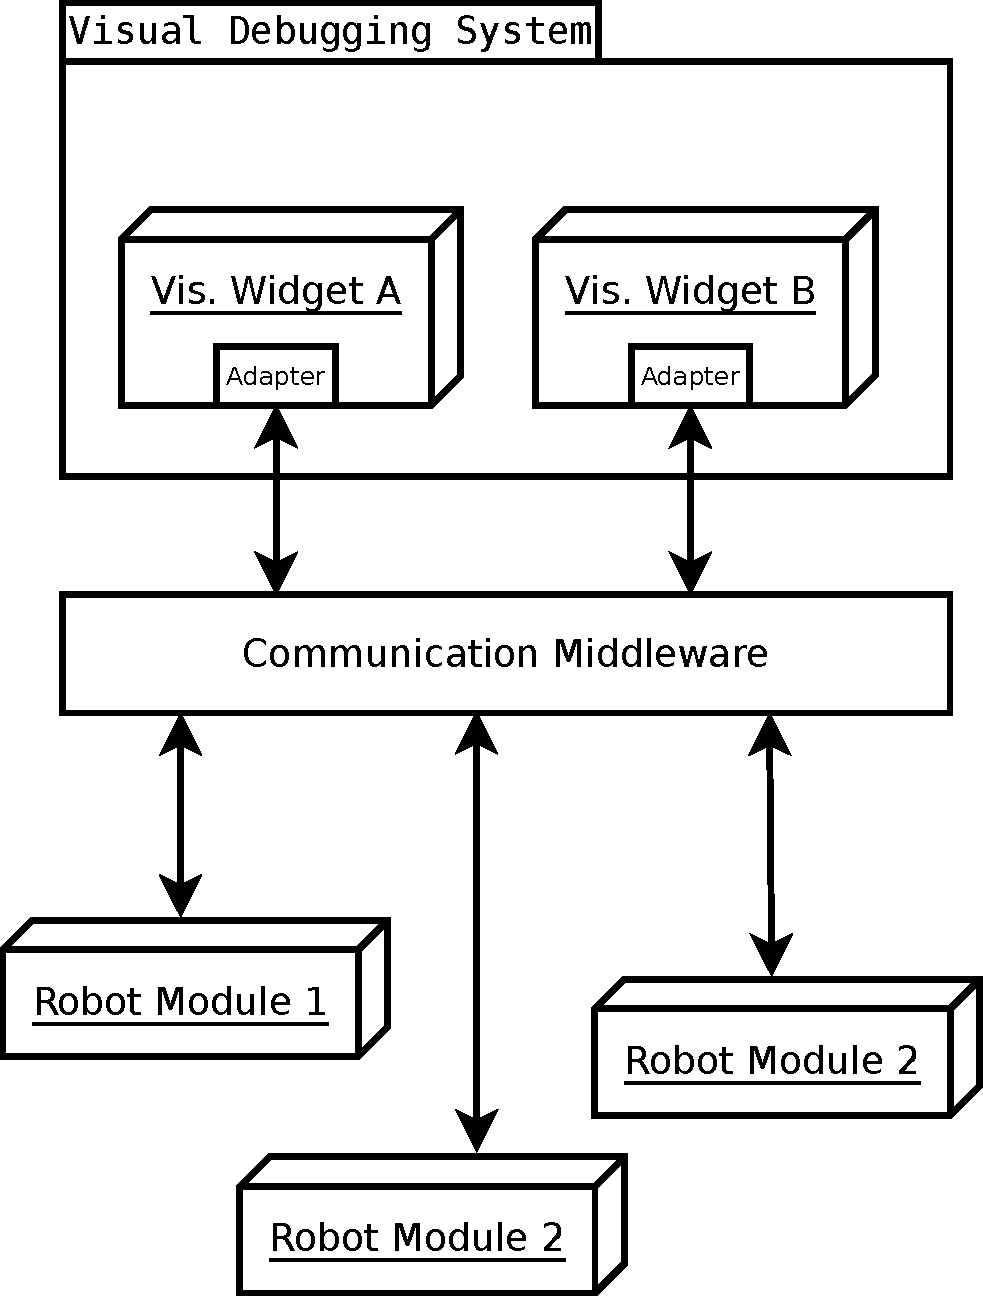
\includegraphics[width=.7\textwidth]{diagrams/communication_diagram}
  \caption{Communication diagram}
  \label{communication_diagram}
\end{figure}

\q
ROS has been examined as an example for a robotic framework with a communication middleware. The publish/subscribe style communication in ROS successfully decouples the sender from the receiver of messages. Since this principle also appears in other frameworks it should be simple to implement an adapter that connects to this communication middleware. If the communication structure is fundamentally diffferent in the target robotic framework, some more work might be required to decouple the visualization from the data collection.

\todo{Should I explain pubsub in detail? class diagram and sequence diagram for example... maybe put that into ros debugging}\q

\subsection{Object Model}
\label{object_model_section}

\begin{figure}%[thpb]
  \centering
  \framebox{
    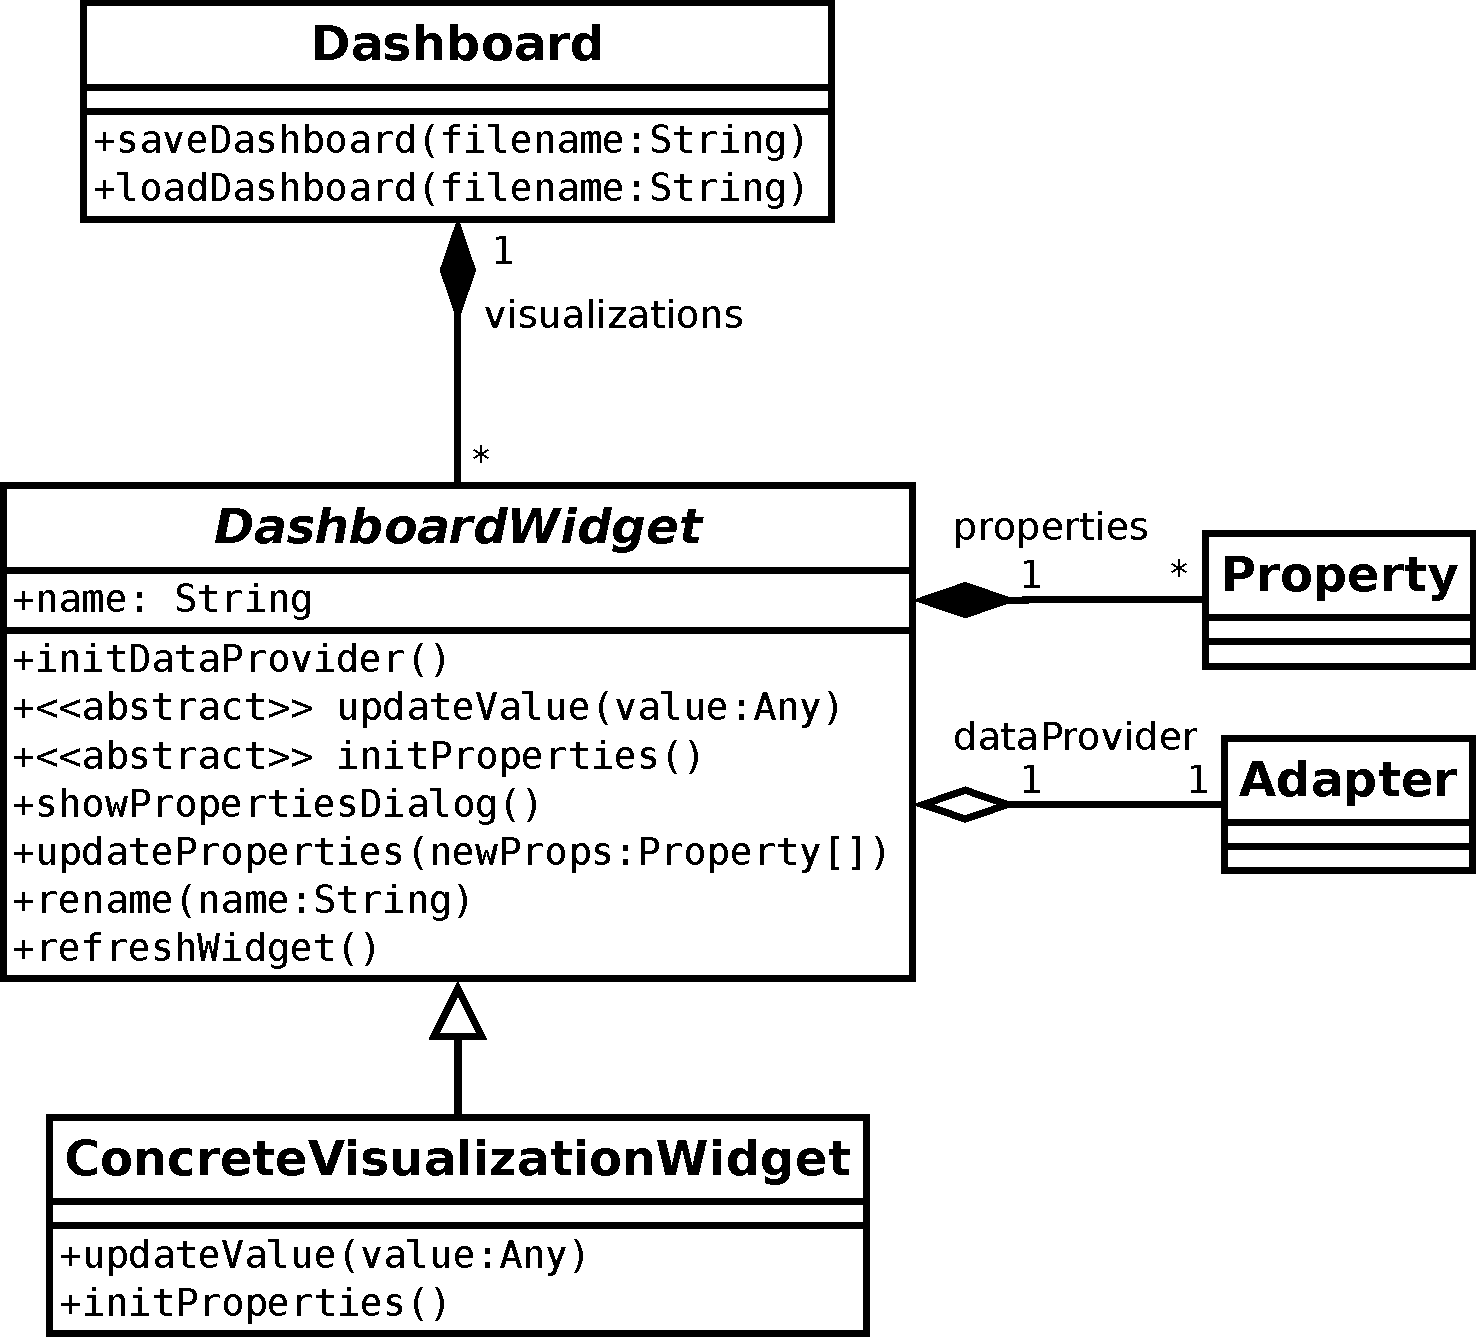
\includegraphics[width=0.9\textwidth]{diagrams/class_overview.pdf}
  }  
  \caption{Extendible object model.}
  \label{class overview}
\end{figure}

The object model shown in Figure~\ref{class overview} was designed to make it easy to extend the debugging system with more visualization widgets. The abstract \textbf{DashboardWidget} class implements the general methods that are the same for every widget. Its internal method structure allows subclasses to overwrite only some parts of functionality, without the need to rewrite most of the other methods. This allows easy integration of a plugin framework at a later stage, where third party widget developers only need to implement the specific parts of the new widget they want to provide and the common parts are handled by the default implementation in \textbf{DashboardWidget}. The class \textbf{ConcreteVisualizationWidget} stands for a possible visualization widget that implements the abstract methods from \textbf{DashboardWidget}. Each visualization widget has to subclass \textbf{DashboardWidget} to make use of \textbf{DashboardWidget}s default implementation framework.

The data provider setup and the properties management are also implemented in the \textbf{DashboardWidget} class, because they will likely be the the same for most widgets. The main reason is to hide the technical details from a third party plugin developer to make his life easier. The plugin developer only needs to specify which properties his widget has in \verb+initProperties()+, the default implementation of \verb+updateProperties()+ saves the new properties and notifies the widget to update the user interface through \verb+refreshWidget()+.
\q The \textbf{DashboardWidget} automatically supports numeric, text and float properties. If more specific properties are needed the plugin developer can overwrite the properties-specific methods in \textbf{DashboardWidget} to provide an implementation tailored to this specific widget.

The \textbf{Adapter} class in Figure~\ref{class overview} can be seen as a black box that takes care of the communication with the communication middleware from the respective robotic framework. The \textbf{Adapter} connects to the communication middleware and waits for new data. If new data is published it notifies the visualization widget to update the value of the widget through \verb+updateValue(value: Any)+.


\subsection{Plugin Architecture}
\label{plugin_architecture_section}
The architecture and object model presented in the previous sections aim to make it easy to extend the visual debugging system with further widgets. To allow third party developers to add their visualizations a plugin architecture will be presented in this section. The plugin architecture allows to add new visualization widgets in form of plugins, without the need to modify the source code directly.

The diagram in Figure~\ref{plugin_architecture_diagram} shows the object design of the plugin architecture. Plugins can be loaded and unloaded through the \textbf{PluginManager} class. The \textbf{PluginManager} class keeps a list of all plugins and populates the toolbox where plugins can be selected from (see Figure~\ref{gui_mockup}). The plugin itself contains the implementation of a visualization widget which is subclassed from \textbf{DashboardWidget} and some additional meta information about the plugin.

\begin{figure}%[thpb]
  \centering
  \framebox{
    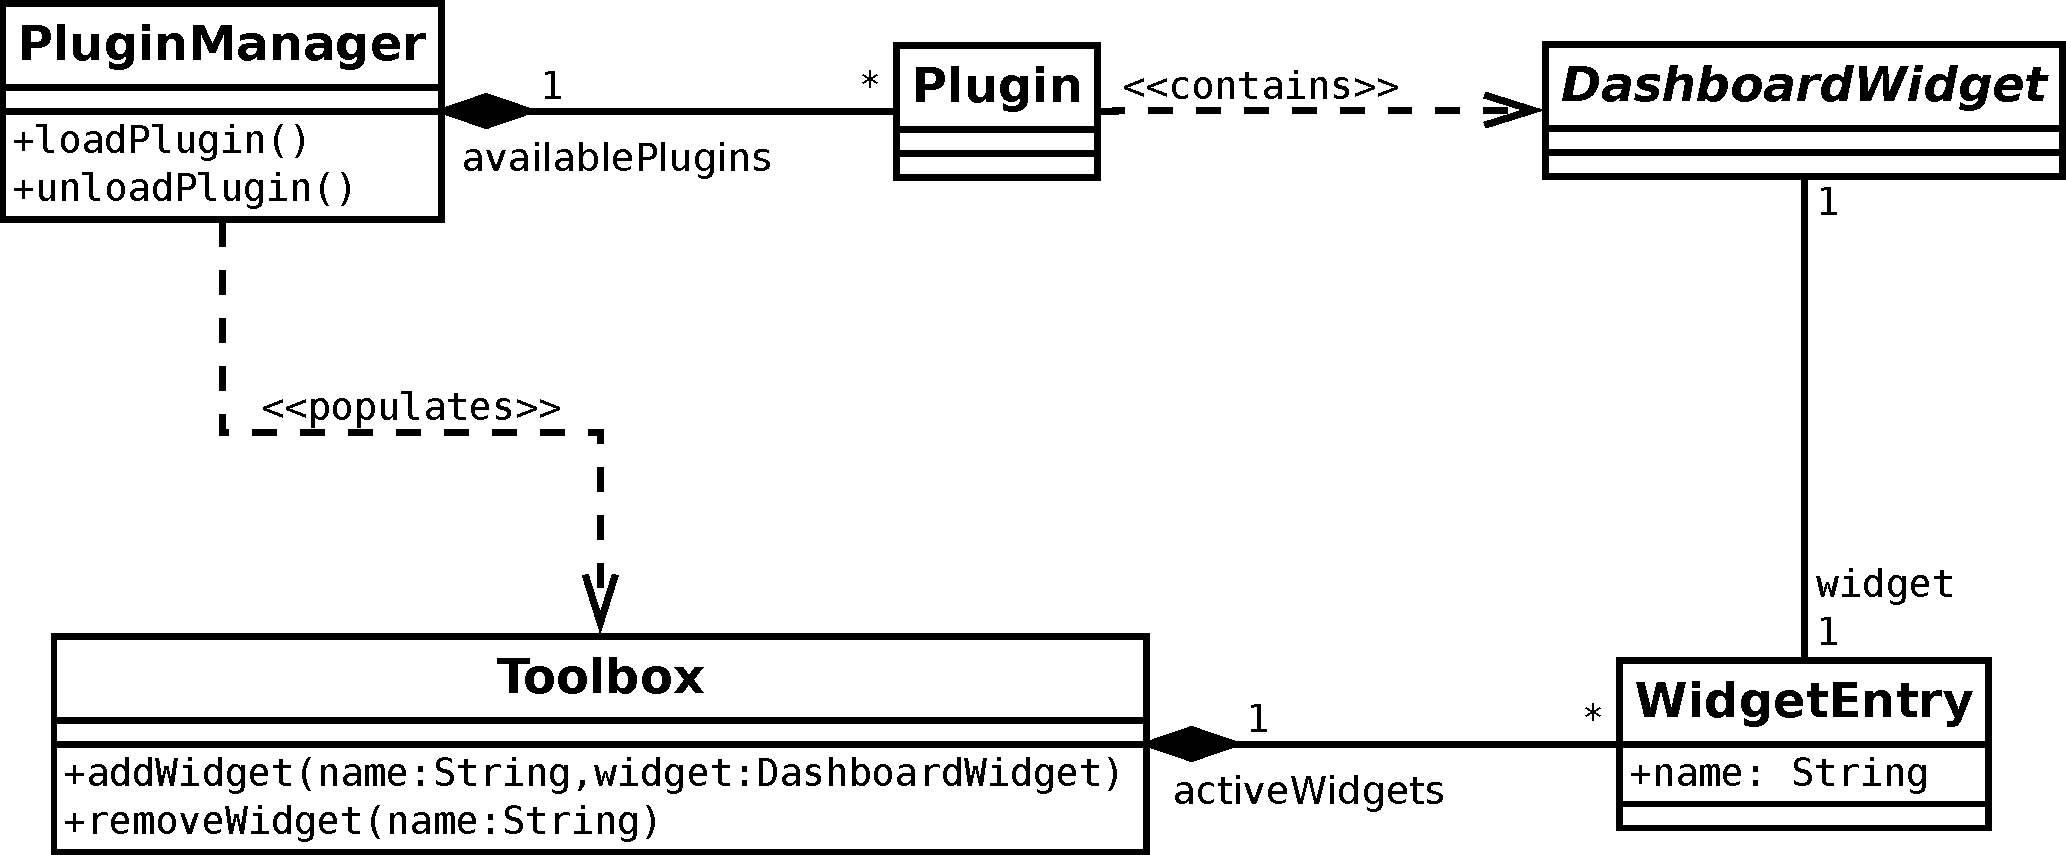
\includegraphics[width=0.9\textwidth]{diagrams/plugin_architecture.pdf}
  }  
  \caption{Possible plugin architecture.}
  \label{plugin_architecture_diagram}
\end{figure}

\chapter{ROSDashboard: A Visual Debugging System for ROS}
\label{rosdashboard}

ROSDashboard is a prototypical implementation of the system design in Chapter~\ref{visual_debugging_system}. The tools target platform is ROS, which provides the communication infrastructure for the tool. The ROS communication middleware is used to connect visualizations in the tool to the respective data published in ROS nodes. The data can be either from existing node-to-node communication or from explicit logging statements that publish data for visualization only.

ROS was chosen as a target platform because it has become a stable and popular robotic framework in recent years \cite{Foote2012}. The publish/subscribe mechanism in ROS provides an easy communication layer that can be accessed using the ROS client API. Since ROS is a modular framework and encourages to encapsulate functionality in several small nodes rather then a single big node, the data on communication channels between existing nodes can be accessed and visualized. The ROSDashboard tool fits good into the existing ROS tool suite and fills the gap between visualization of complex data in RViz (see Section~\ref{rviz}) and text only debugging with ROS logging mechanism and rxconsole.

Although the design in Chapter~\ref{visual_debugging_system} does not imply the use of a specific robotic framework, some of the architectural decisions were driven by the ROS architecture which was examined during the initial survey of existing debugging tools and practices in robotics. As a result the implementation of ROSDashboard did not require a lot of glue code to connect to the communication infrastructure. If another robotic framework is chosen as target platform for an implementation, more work might be required to access the data from the robotic application. This highly depends on the existing communication infrastructure of such a robotic framework and whether it can be accessed transparently without the robot module knowing about the visualization.

\todo{This chapter introduces}

%rosdashboard is a prototypical implementation of the system presented in Chapter~\ref{visual_debugging_system} for the ROS middleware / framework. ROS was chosen as middleware because the simple publish/subscribe mechanism allowed to connect to topics transparently without the other party explicitly knowing about the visualization tool.

[Not sure if this is possible in other frameworks, if not it could be stated that more work is needed for those frameworks in order to make communication transparent. In general I can argue that ROS fits the requierements best, the system design was not intended to fit every framework but was developed without compromises current systems might have]

[I'm not sure how to write this chapter: can I have a section "why ROS?", "how the requirements are met?", ...?] ---> this should be written in the introduction for this chapter: ROS was used because it has many users, an easily accesible communication structure, a tool landscape (?) where such a tool would fit in well (recent surge of graphical tools like rxdeveloper, rqt, other dashboards).

\parbox{.8\linewidth}{
[from icra paper, needs some changes]

ROSDashboard, the tool presented in this work, aims to support the developer during debugging by visualizing data in a graphic way and thus eliminating the cognitive effort needed to parse and interpret text based logging messages. While most of the currently available visualization tools in robotics focus on spatial data to help understand the robot and the environment in which it runs \cite{Collett2010, Quigley2009}, rendering of abstract data is still uncommon. ROSDashboard provides a dashboard interface to robot developers, which they can populate with graphical widgets to visualize all kinds of data from the robot. The dashboard can be customized to display widgets according to the current robot hardware and development stage. It can be used to visualize data during debugging as well as monitor data during the normal execution of the robot. This means ROSDashboard is a tool that a) can be adapted to many different use cases and b) allows the developer to choose the widgets he or she thinks represent the data best, according to their mental model and the meaning of the data. The tool is based on ROS (Robot Operating System) which abstracts from specific robot hardware and takes care of inter process communication \cite{Quigley2009}.
}

%%%%% Robot Operating System ROS %%%%%%
\section{Robot Operating System (ROS)}
The Robot Operating System (ROS) is an Open Source framework for complex robotic systems. The first work on ROS was done as part of the STanford Artificial Intelligence Robot (STAIR) in 2007 \cite{Quigley2007}. The original software library was called \emph{Switchyard} and had been developed at Stanford. Later the library was refined and generalized to also suit the requirements of the Personal Robot Program at Willow Garage\footnote{www.willowgarage.com} \cite{Quigley2009}. The resulting general framework has been released as Open Source \cite{Quigley2009} and this section gives a short overview over the most important principles in ROS.

\begin{figure}[ht]
\centering
\subfigure[Stanford's STAIR]{
	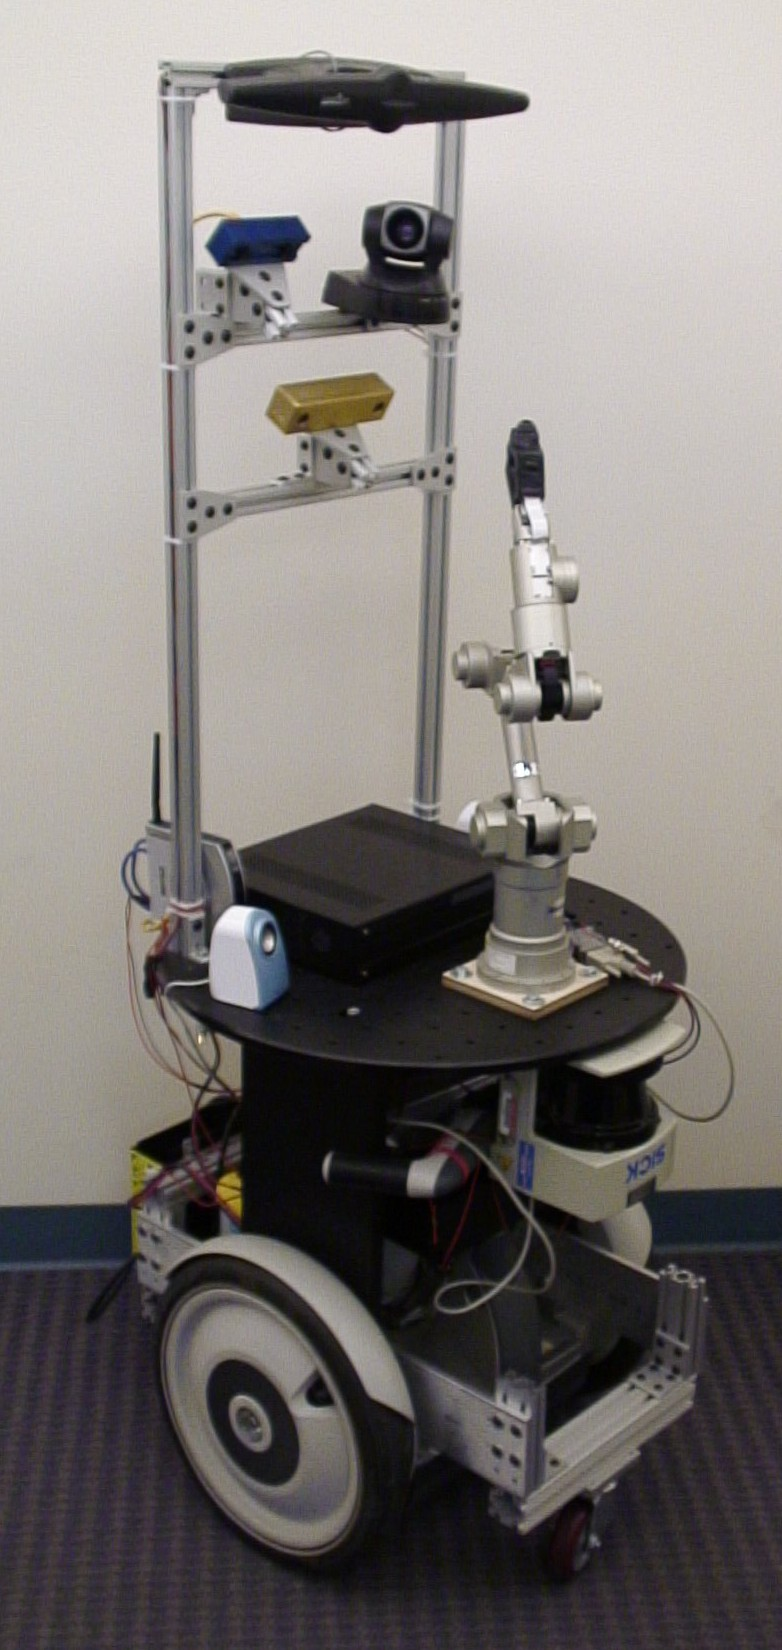
\includegraphics[height=8cm]{img/stair}
}
\subfigure[Willow Garage's PR2]{
	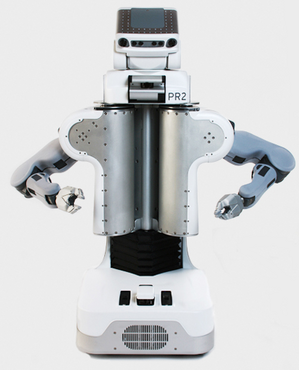
\includegraphics[height=8cm]{img/pr2}
}
\end{figure}

ROS has grown significantly in the last years, it has an active community backing the project and supports many of the currently available robots \cite{Foote2012}. It was developed to abstract from the hardware of the robot and make it easier to create modular robot software, which can run on different robots and on different machines. The modular approach makes development easier, because the work can be divided amongst different developers or development teams. This also allows the developer to change only small parts of a complex system, without the need to build and re-deploy the whole system.
The modules in ROS are called \emph{nodes} and several nodes executed together are called a \emph{stack}. ROS \emph{packages} bundle nodes and stacks and are used to make software modules available to other developers. Everyone can create their own package which can be indexed by ROS so that their software modules can be found, downloaded and used by other developers. There exist many packages, nodes and stacks with implementations of algorithms for some of the most common problems in robotics (e.g. navigation, localization, joint movement, etc.) and they can easily be (re-)used.

The communication between ROS nodes is either asynchronous through a publish/subscribe mechanism or synchronous through services. Nodes can send messages by publishing a message on a topic and receive messages by subscribing to that topic. This mechanism is flexible and decouples the sender from the receiver. A publisher node does not need to know if there are other nodes listening and vice versa. For synchronous communication and guaranteed delivery of messages, services can be invoked. The routing for publish/subscribe messages is established during runtime through the ROS core. The communication between nodes is one of the main sources for debugging data when debugging a ROS application. The same communication framework is also used for the logging mechanism in ROS, which publishes messages to the special purpose topic \emph{/rosout}.

\todo{Overview over this section}

\todo{explain why ros was chosen?}

\todo{list some tools and recent projects that have influenced the tool. For example the rxdeveloper tool and the survey in Muellers2012, RQT and other dashboards recently developed. Highly related to the choice of making a tool for ros.}

\subsection{ROS Publish/Subscribe Mechanism}
\todo{explain the pubsub mechanism in detail? reference here from the system design section which mentiones pub/sub}

\subsection{Related ROS Tools}

\subsubsection{rxplot, rxconsole, rxbag?}
\todo{decide whether to keep this subsection or not}
rxplot is a graphical tool which can plot values from topics on a Cartesian coordinate system. The tool takes data from a published ROS topic and prints it on a time graph. The tool can be configured to visualize several graphs in one go, which makes it easy to compare values and data streams.

[rxplot screenshot, there is not much more to say]

\subsubsection{RQT - ROS GUI}
--> remove from debugging section, not related to debugging. can be introduced in rosdashboard when reasons for the choice of ros are presented (rosdashboard integrates well with other tools in the ros environment and recently many graphical tools were developed)

\subsubsection{rxDeveloper}
[\textbf{outline, results of the survey, importance for this work}]
\cite{Muellers2012}

[Not really debugging, this might go somewhere else? Maybe not a full subsecion but only a couple of sentences that summarize the results and why it is important for this work]

%%%%% Implementation Details %%%%%%
\section{Implementation Details}

\subsection{Topic Introspection}

\begin{figure}[thpb]
  \centering
  \framebox{
    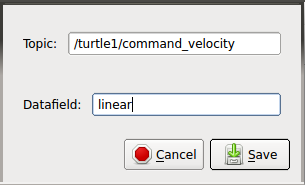
\includegraphics[scale=0.8]{img/topic_setup.png}
  }  
  \caption{Screenshot of the topic setup dialog. [re-do screenshot with rosdashboard in background]}
  \label{topic setup screenshot}
\end{figure}

ROS topics were originally not designed and developed as something the user or developer chooses graphically: They are usually created, configured and used in the source code. ROSDashboard exposes the topic setup in a graphical user interface every time a new widget is added to the dashboard. To make this as easy as possible and without much overhead, a technical solution was chosen to reduce the number of fields to be set during the topic subscription setup. Normally you have to select a topic name and a message data type. The data type can be one of the standard message types like Float, Integer, String and Boolean or a more complex message type which contains more information in a structured message. To access one data element of a message the ``datafield'' field was introduced in the graphical interface. Figure~\ref{topic setup screenshot} shows an exemplary topic setup configuration to access the linear velocity of the \emph{/turtlesim/Velocity} message published to the topic \emph{/turtle1/command\_velocity}. Using Python's duck typing and the \emph{rostopic} module it was possible to avoid the complexity of dynamically binding message type classes during runtime and detect the message type automatically. If a topic is not yet published and thus the message type of this topic is not defined yet, the method call to \emph{rostopic} will block until the message type becomes available. To avoid blocking of the user interface a listener thread was implemented to wait until the message type for a topic becomes available (see Figure~\ref{topic subscription}). Avoiding to manually ask the user for a message type makes the configuration of widgets easier and faster for the user, it also keeps the implementation significantly simpler, because no dynamic binding of message type classes during runtime is needed.

\begin{figure}[thpb]
  \centering
  \framebox{
    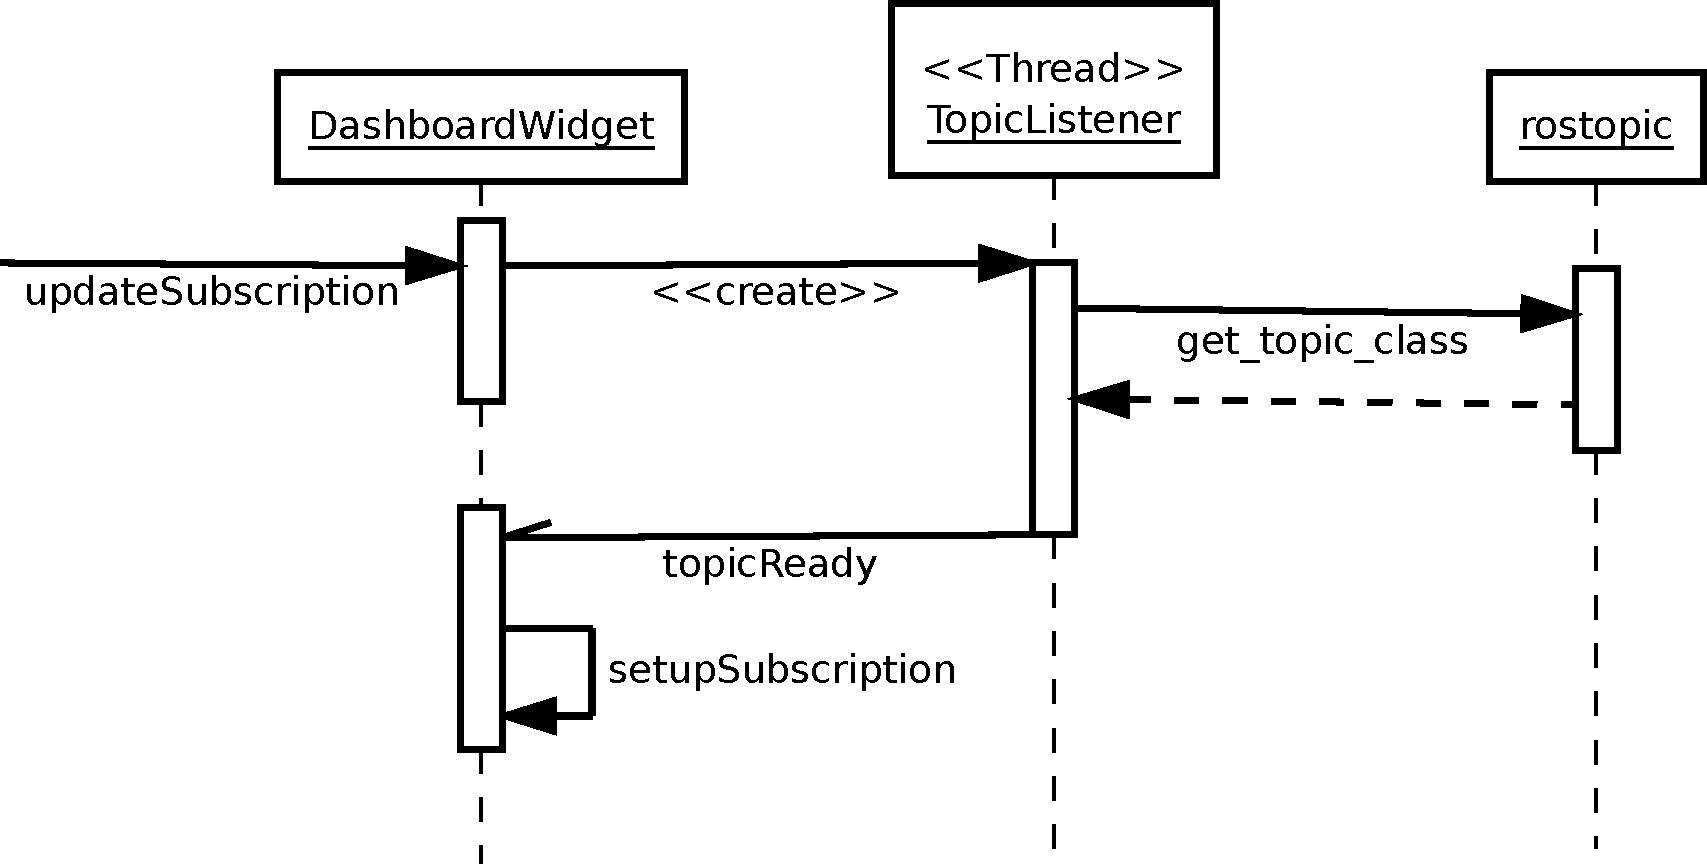
\includegraphics[scale=0.4]{diagrams/topic_subscription.pdf}
  }  
  \caption{Exemplary flow of events for asynchronous topic subscription setup.}
  \label{topic subscription}
\end{figure}

\subsection{User Interface}
The user interface was implemented based on the early interface designs from Section~\ref{graphical_user_interface}. The main window consists of the dashboard canvas where visualization widgets can be positioned freely and a toolbox where all the available visualization widgets can be selected. The visualization widgets can be positioned on the dashboard by "Drag\&Drop" from the toolbox. Figure~\ref{screenflow} shows a series of screenshots, depicting every step necessary to put a visualization widget on the dashboard: First the desired widget needs to be selected in the toolbox and dragged to the dashboard. When the widget is dropped on the dashboard, the configuration dialog opens automatically where the developer can select to which topic and datafield the visualization widget should connect to. This dialog can be re-opened later from the context menu of the widget, as well as the rename dialog and the properties dialog. It was deliberately chosen to separate the dialog for setting up a topic connection and the dialog for other settings of the widget. This separation of concerns keeps the data provider setup encapsulated in its own dialog, which makes it easier to exchange the data provider if necessary. To remove a widget from the dashboard, simply drag it to the bottom of the dashboard where a special drop zone deletes the widget from the dashboard.

\begin{figure}[ht]
\centering
\subfigure[Empty dashboard]{
    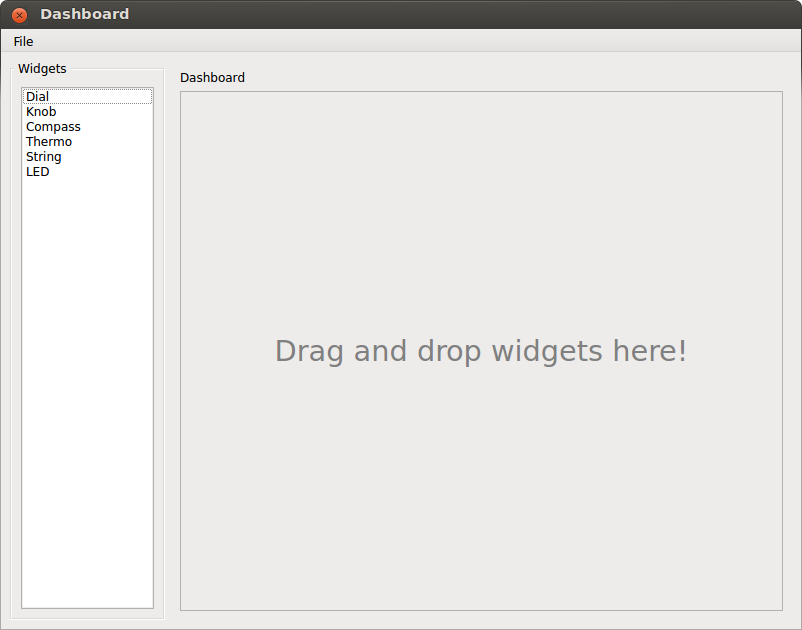
\includegraphics[width=0.45\textwidth]{img/screenflow1.png}
}
\subfigure[Dragging widget to dashboard]{
    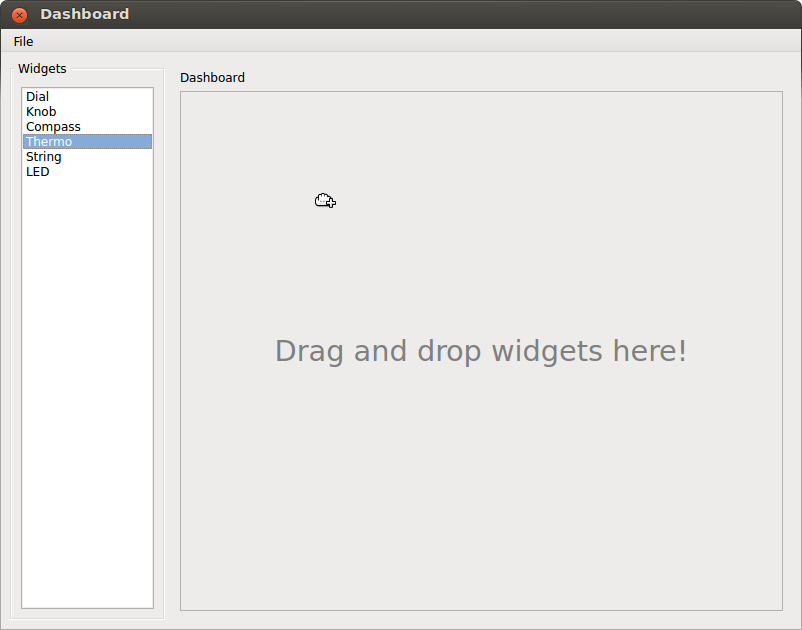
\includegraphics[width=0.45\textwidth]{img/screenflow2.png}
}
\subfigure[Configure subscription on drop]{
    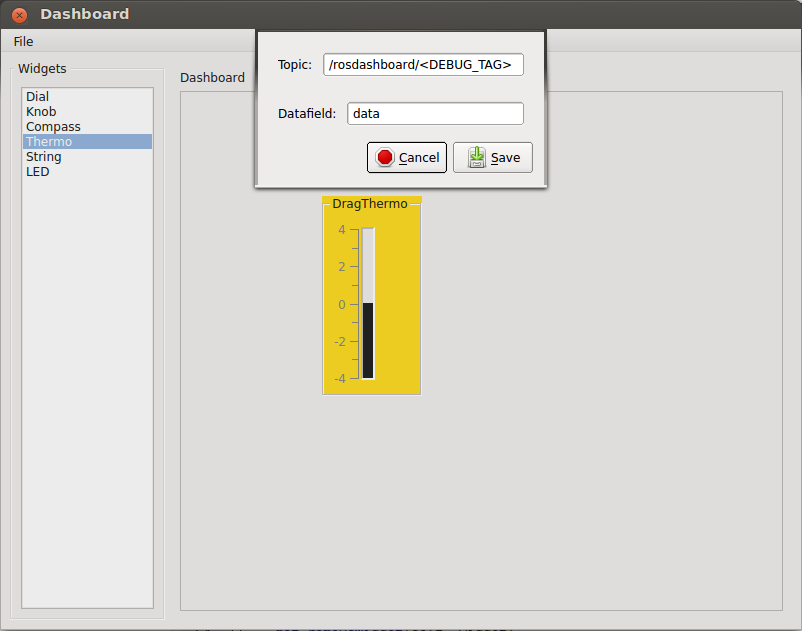
\includegraphics[width=0.45\textwidth]{img/screenflow3.png}
}
\subfigure[Context menu]{
    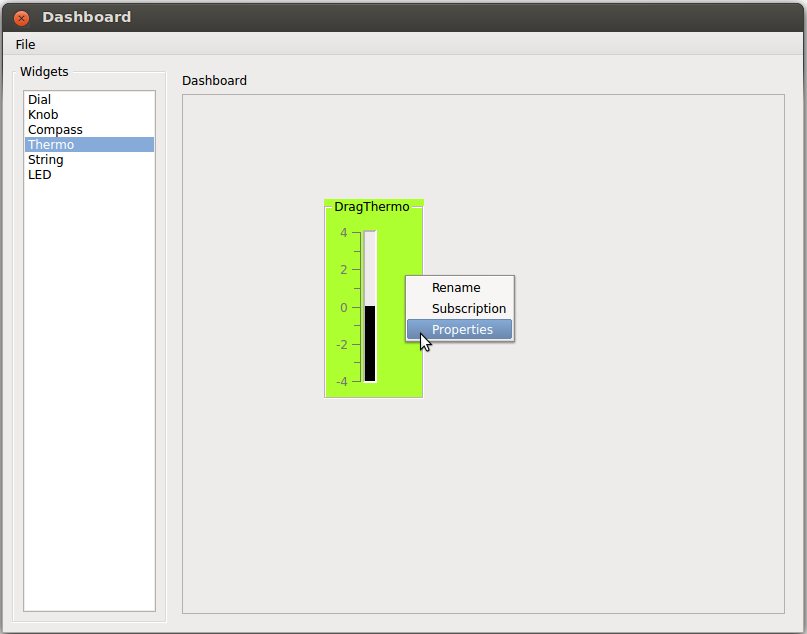
\includegraphics[width=0.45\textwidth]{img/screenflow4.png}
}
\subfigure[Properties dialog]{
    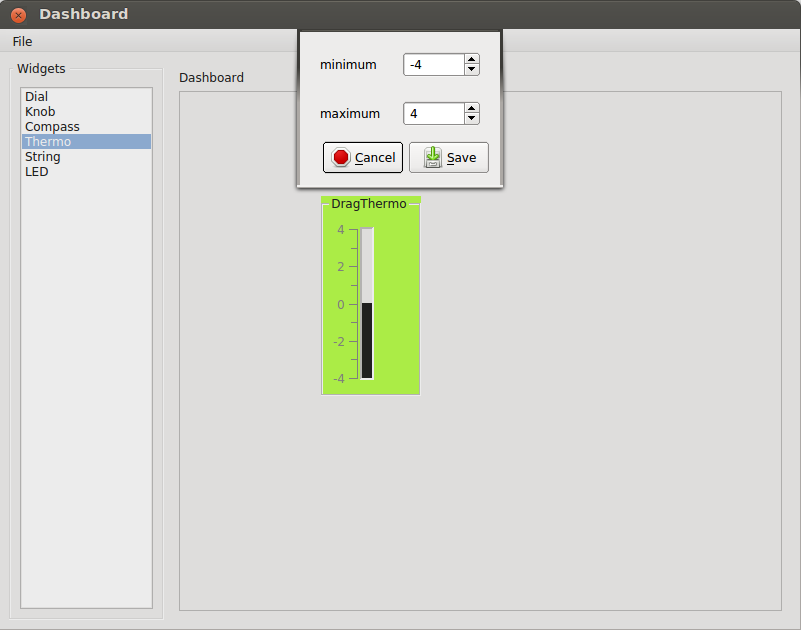
\includegraphics[width=0.45\textwidth]{img/screenflow5.png}
}
\subfigure[Drag to bottom to remove]{
    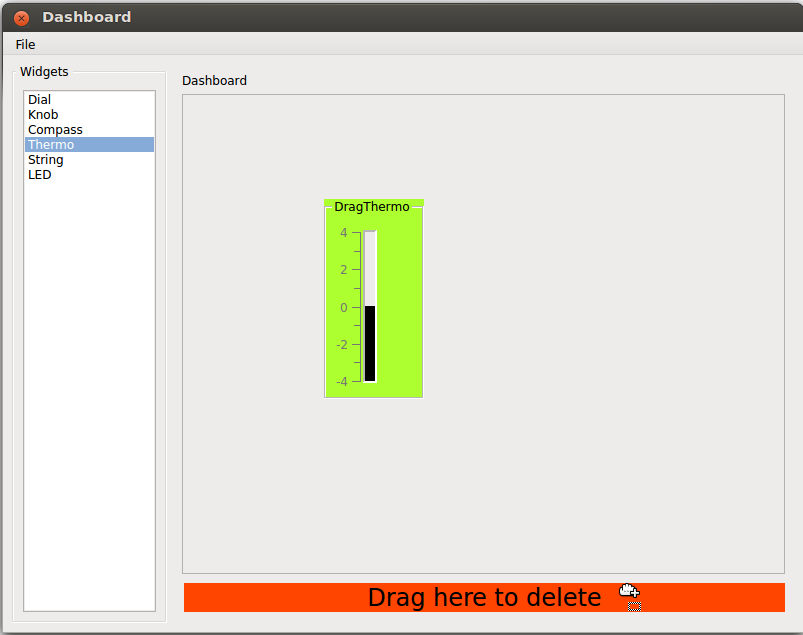
\includegraphics[width=0.45\textwidth]{img/screenflow6.png}
}
\caption{Screenflow when adding and removing widgets from the Dashboard.}
\label{screenflow}
\end{figure}


The widgets background has two different colours to provide additional feedback to the developer whether the visualization is connected to a topic or not. When the configured topic for a visualization widget is not available yet, the background of the widget is coloured in orange. Once the topic becomes available the widget changes its background colour to green. This mechanism only checks the availability of a topic on the communication middleware, it does not time out if a topic has been without any messages for a while. Figure~\ref{colour_widgets} shows the two different colour states of a widget.

\begin{figure}%[thpb]
  \centering
  \framebox{
    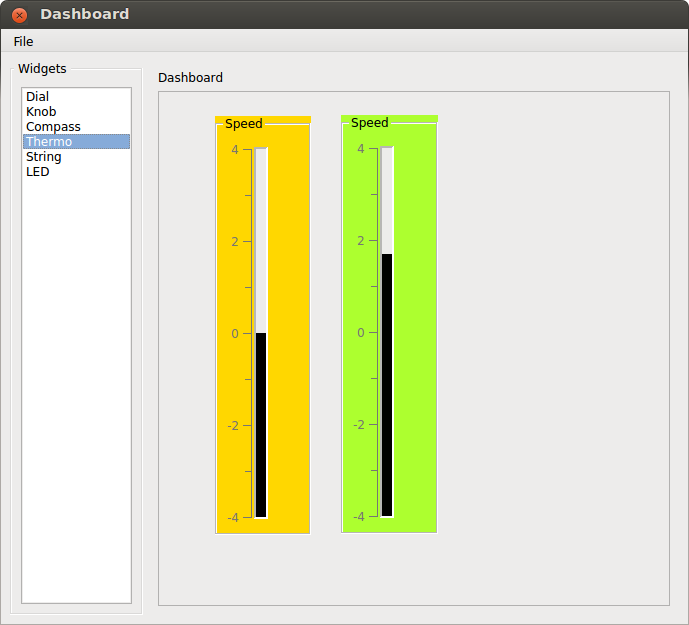
\includegraphics[width=0.9\textwidth]{img/colour_states.png}
  }  
  \caption{Different colour cues provide additional information.}
  \label{colour_widgets}
\end{figure}

Figure~\ref{all_widgets} shows a dashboard with every currently available widget on it. The currently implemented widgets are:
\begin{description}\itemsep2pt
\item[Dial] A dial widget similar to the speedometer on the dashboard of a car or motorbike.
\item[Knob] The knob is similar to the dial but is usually smaller. While it is originally often used as input widget, we use it only to visualize numeric data.
\item[Compass] The compass is a 360 degree display which can be used e.g. to visualize orientation.
\item[Thermo] The thermo is a horizontal progress bar with a scale similar to a thermometer.
\item[String] The string widget is a text field to show logging messages or other textual information.
\item[LED] The LED widget can visualize boolean data, the LED is either green or red.
\end{description}

\begin{figure}%[thpb]
  \centering
  \framebox{
    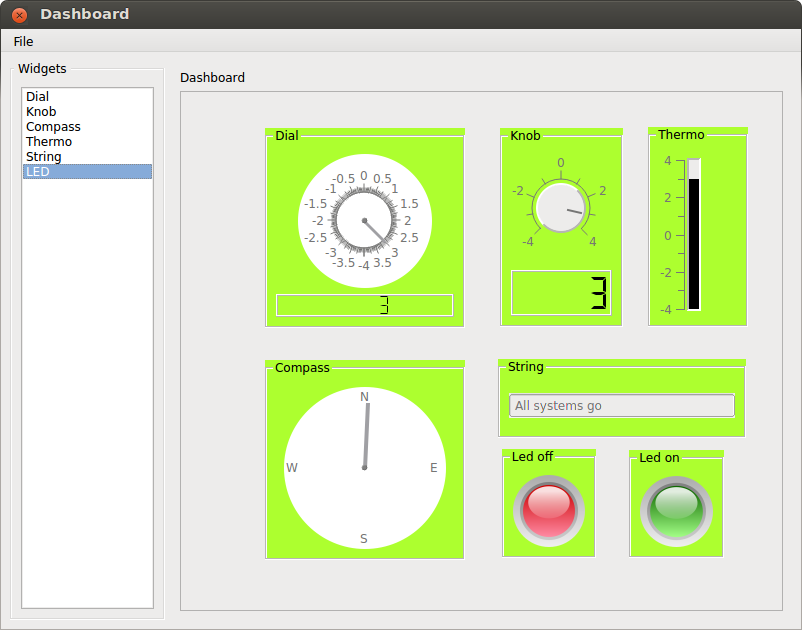
\includegraphics[width=0.9\textwidth]{img/all_widgets_active_screenshot.png}
  }  
  \caption{Dashboard with all currently available widgets.}
  \label{all_widgets}
\end{figure}

\subsection{Data Format}
To share the configuration of a dashboard a save and restore mechanism was integrated. ROSDashboard can save a current configuration of the dashboard to a file which can be used to save the current work and to provide other developers with the same interface. For the prototype all data is stored in a text-based file in JSON (JavaScript Object Notation) \cite{JSON} format. Listing~\ref{json_example} shows an example dashboard configuration represented as JSON, which can be stored in a file. The example contains one visualization widget which is a thermometer widget and is set up to visualize data from the linear field of the \emph{/turtle1/command\_velocity} topic.

\begin{lstlisting}[frame=single,caption={Example dashboard configuration in JSON.},label=json_example]
{
  "widgets": [
    {
      "width": 105,
      "height": 197,
      "name": "Linear Velocity",
      "posX": 50,
      "posY": 25,
      "subscription": {
        "topic": "/turtle1/command_velocity",
        "datafield": "linear"
      },
      "type": "DragThermo",
      "properties": [
        {
          "type": "numeric",
          "name": "minimum",
          "value": -4
        },
        {
          "type": "numeric",
          "name": "maximum",
          "value": 4
        }
      ]
    }
  ]
}
\end{lstlisting}

This feature could also be used by robot software and hardware manufacturers to provide a dashboard for a specific module or piece of robot hardware. The dashboard configuration can be made available as part of the module's documentation and represents a easy way to explore the possibilities of a new hardware or software module.

\subsection{Plugins}
Reference to the plugin framework section in Chapter~\ref{visual_debugging_system} and that such a system was not yet implemented in ROSDashboard [can I say: due to the time constraints of this work?], but the necessary measures have been taken to allow this in the future. Show some details about an example widget and what methods it overwrites.

\subsection{Adding a Visualization Widget}
\todo{Explain how the plot widget was added --> this is some kind of evaluation already, should this go into the showcase? conclusion? where else}

\todo{fix inconsistent method names from system design to implementation?}

\begin{figure}%[thpb]
  \centering
  \framebox{
    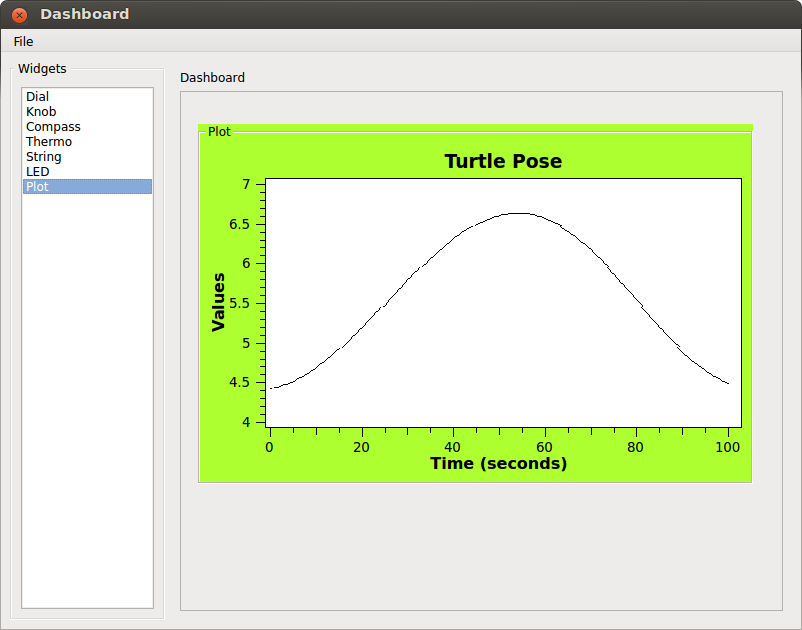
\includegraphics[width=0.9\textwidth]{img/plot_widget.png}
  }  
  \caption{The newly created plot widget in action.}
  \label{plot_widget}
\end{figure}

Adding new visualization widgets to ROSDashboard is easy. The abstract \textbf{DashboardWidget} class (see Figure~\ref{class overview}) handles most of the generic things a widget should implement. As part of a first evaluation step a new visualization widget was added to the dashboard: A plot widget that plots values on a Cartesian coordinate system (see Figure~\ref{plot_widget}). To implement the widget, a new class called \textbf{DragPlot} was created. The class inherits the basic implementation from \textbf{DashboardWidget} and only needs to implement the plot specific methods. Upon initialization of \textbf{DragPlot} the user interface part of the widget is created. The class implements the two abstract methods \verb+updateValue+ and \verb+initProperties+ from \textbf{DashboardWidget}. \verb+updateValue+ updates the graphical part of the widget and \verb+initProperties+ adds two properties to the widget: plot name and update rate in milliseconds. This requires only two lines of code, see Listing~\ref{init_props}.

\begin{lstlisting}[frame=single,caption={Implementation of initProperties in DragPlot.},label=init_props,language=Python]
# property keys
TITLE = 'Plot title'
RATE = 'Refresh rate (ms)'

def initProps(self):
  self.props[self.TITLE]=WidgetProperty('text', 'Plot title')
  self.props[self.RATE]=WidgetProperty('numeric', 500)
\end{lstlisting}

The default implementation in \textbf{DashboardWidget} is capable of automatically generating a user interface for those simple properties. When the properties are updated in the properties dialog, a callback is used to notify the \textbf{DragPlot} class. The callback implementation to refresh the widget is shown in Listing~\ref{prop_callback}. It updates the title of the plot and starts a new timer which updates the plot in a given interval.

\begin{lstlisting}[frame=single,caption={Implemented callback in DragPlot.},label=prop_callback,language=Python]
def updateWidget(self):
  #update the widget properties
  self.qwtPlot.setTitle(self.props[self.TITLE].value)

  if (self.currentTimerId != 0):
    self.qwtPlot.killTimer(self.currentTimerId)
    self.currentTimerId = 0

  self.currentTimerId = self.qwtPlot.startTimer(
                             self.props[self.RATE].value)
\end{lstlisting}

The plot itself is a \textbf{QwtPlot} widget from the popular QWT widget library\footnote{\url{http://qwt.sourceforge.net/}}. To customize the plot widget, \textbf{QwtPlot} was subclassed in \textbf{DataPlot}. The \textbf{DataPlot} class exposes two methods: \verb+addValue(value)+ and \verb+timerEvent()+. The \verb+addValue(value)+ method is used in the implemented abstract method \verb+updateValue(value)+ from \textbf{DashboardWidget} and adds a new value to the plot. \verb+timerEvent()+ is a callback that gets triggered regularly, how often depends on the update rate which can be set in the properties of the widget.

The last step to add the new visualization widget to ROSDashboard is to add it manually to the list of available visualization widgets which appears in the toolbox left of the dashboard canvas. This example shows how easy it is to add a new widget to ROSDashboard. A plugin architecture would make it even easier, since the last manual step is not required and widgets could be dynamically loaded as plugins.

\subsection{API}
\label{api_section}
The current ROS logging framework publishes the log messages on the special purpose topic \emph{/rosout}, but converts everything to a String before the transmission. Since those logging messages are text based, valuable information about the type of the data is lost. To use the data for visualization, the type information must be kept. Thus a set of convenience methods were exposed in the ROSDashboard API (Listing~\ref{api_calls}) to provide a simple interface to publish data for the visualization. The interface is similar to the logging API exposed in the ROS client libraries and basically wraps the ROS specific methods to publish data on a topic. Listing~\ref{api_implementation} shows the simple implementation of the \verb+logint+ API method.

\begin{lstlisting}[frame=single,caption={ROSDashboard API methods.},label=api_calls,language=Python]
# log arbitrary data,
# try to find the data type with introspection
api.log(tag, data)

# log string message
api.logstring(tag, msg)

# log integer value
api.logint(tag, value, msg_type=Int32)

# log float value
api.logfloat(tag, value, msg_type=Float32)

# log complex data with datatype
api.logdata(tag, data, msg_type)
\end{lstlisting}

\begin{lstlisting}[frame=single,caption={Implemented logint API method.},label=api_implementation,language=Python]
def logint(tag, value, msg_type=std_msgs.msg.Int32):
    """
    publishes a integer value to the /rosdashboard/<tag> topic
    Be careful to use only valid tags, ROS does not allow
    dashes and dots in the topic name.
    
    The default integer message type is std_msg.msg.Int32
    """
    pub = rospy.Publisher('/rosdashboard/' + tag, msg_type)
    pub.publish(msg_type(value))
\end{lstlisting}

The API methods shown in Listing~\ref{api_calls} can be used like logging statements to emit data for visualization. The \verb+TAG+ parameter is used to identify the data when the visualization widgets are set up. Internally the data is published as a message on a ROS topic. The topic name consist of the ROSDashboard specific prefix \emph{/rosdashboard/} and the tag given as parameter. Listing~\ref{example_api_call} shows an example use of the API to publish a integer value with the tag "proximity". The value "7" will be published on the ROS topic \emph{/rosdashboard/proximity} and can be visualized with a widget in ROSDashboard that points to the respective topic name and accesses the "data" datafield of the message.

\begin{lstlisting}[frame=single,caption={Example API usage.},label=example_api_call,language=Python]
import rosdashboard

rosdashboard.logint('proximity', 17)
\end{lstlisting}

Although this solution proved to be a useful way to expose data during debugging, it might not be feasible for a bigger project because it introduces a new dependency to ROSDashboard. Since the API is only a set of convenience methods that publish data on ROS topics, data can also be published using the same ROS methods the API uses directly in the target application. Other possible solutions will be discussed as future work in Chaper~\ref{future_work}.

\chapter{Case Study}
\todo{Describe the case study: two different steps, the first one without code modification (monitoring of existing communication channels), the second one where code is actually modified to emit special debugging messages (can be done with rosdashboards api or manually).}

\todo{Talk to Jamie Diprose about his Nao work with ROS (probably better than the turtlesim example from the ICRA paper), or see if rosbag data can be found and build showcase on top of the rosbag data.}

Although the current implementation is a prototype, it has all the features that were initially planned. The implementation is running stably and first attempts to use it as a debugging tool have been made. ROSDashboard is ready to be used for the development of robot applications and can be used for further evaluations (see Section~\ref{future_work}).

Figure~\ref{showcase} shows a simple showcase scenario: ROSDashboard is running alongside the \emph{turtlesim\_node} node which is used in many examples in the ROS tutorials\footnote{http://www.ros.org/wiki/ROS/Tutorials}. It monitors the values for linear and angular speed which are published by the \emph{turtle\_teleop\_key} node to control the turtle simulation. The String widget is configured to display messages from \emph{/rosout}, which in this example shows a warning when the turtle hits a wall.
For the purpose of this small showcase, there was no need to modify the turtlesim source code. The only topics used by the showcase scenario are topics that are already used to control the turtle in the simulation and to display warnings.

\begin{figure}[thpb]
  \centering
  \framebox{
    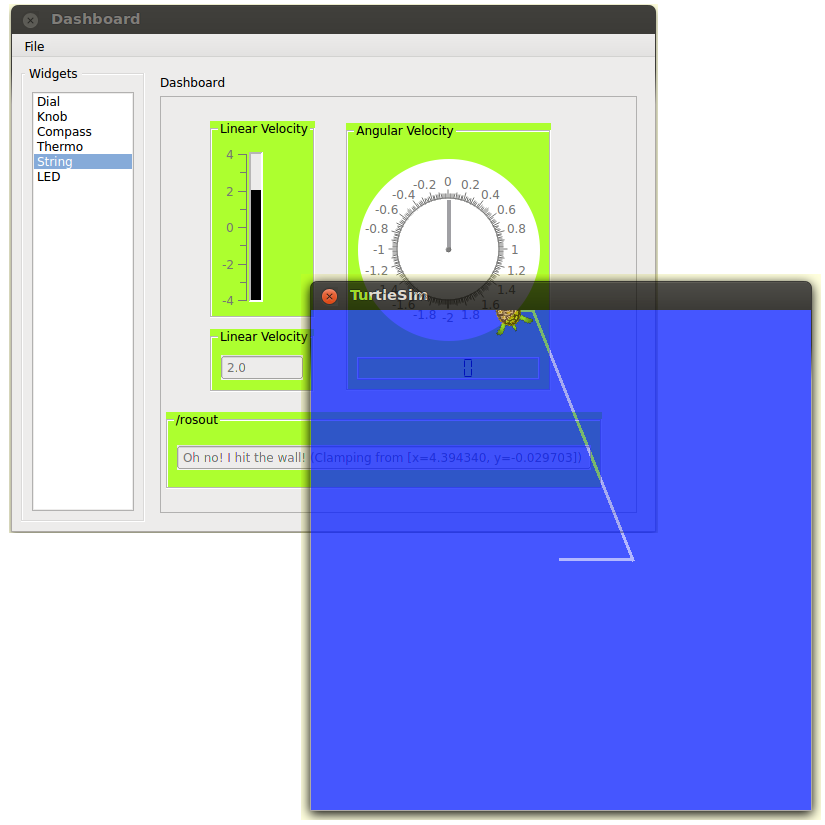
\includegraphics[width=0.9\textwidth]{img/showcase3.png}
  }  
  \caption{ROSDashboard running alongside turtlesim\_node.}
  \label{showcase}
\end{figure}

Figure~\ref{rosgraph_simple} shows the ROS computation graph during the execution of the showcase scenario. It shows how ROSDashboard is connected to the nodes which are debugged. The topics needed for the showcase are \emph{/turtle1/command\_velocity} for the linear and angular velocity and \emph{/rosout} for warnings when the turtle hit the wall.

\begin{figure}[thpb]
  \centering
  \framebox{
    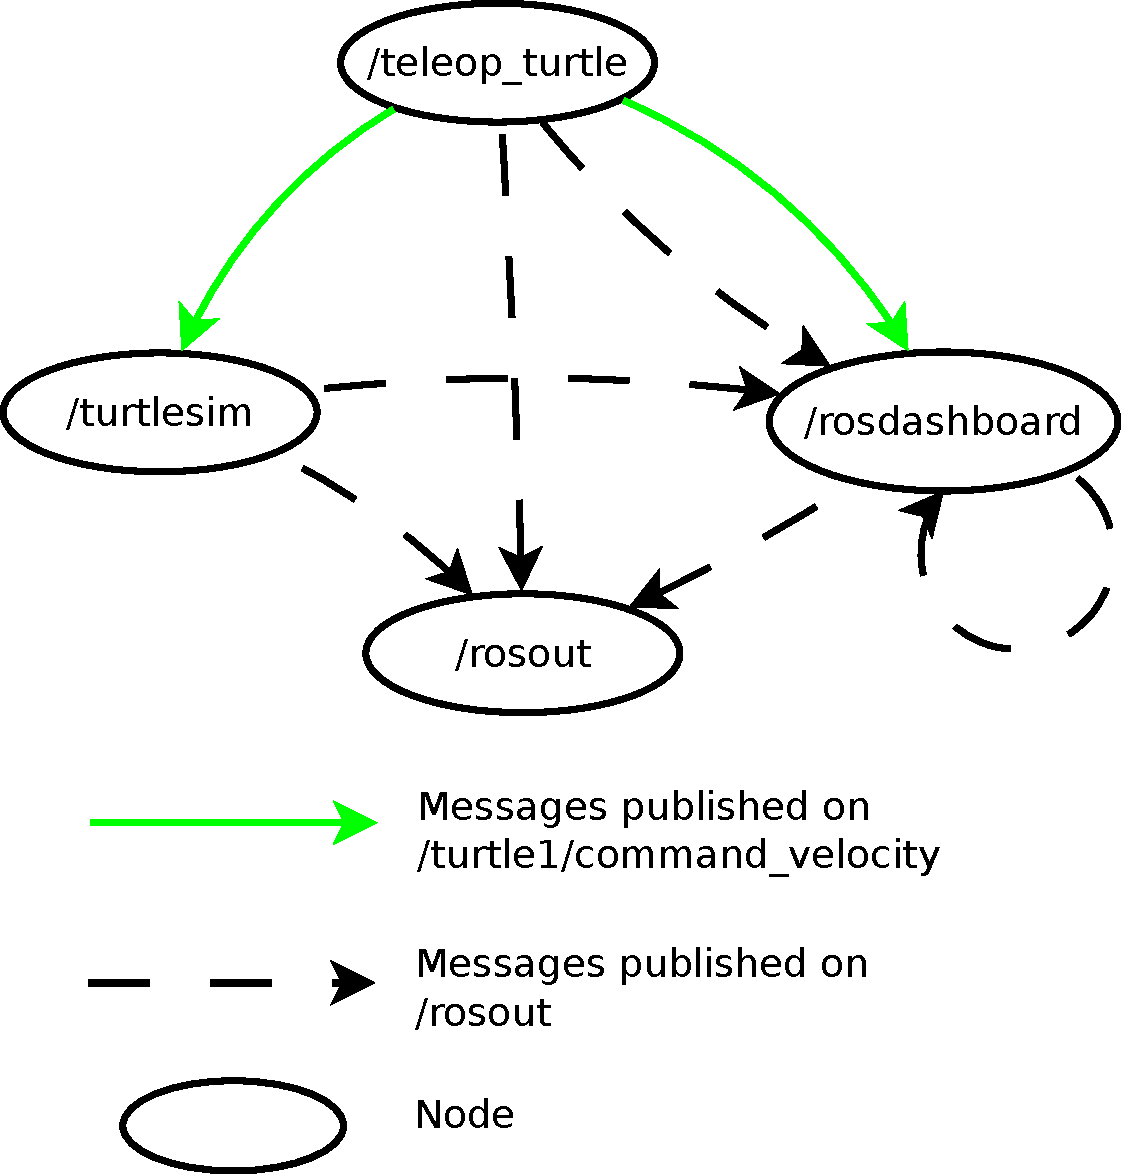
\includegraphics[width=0.7\textwidth]{diagrams/rosgraph}
  }  
  \caption{Simplified ROS computation graph with ROSDashboard.}
  \label{rosgraph_simple}
\end{figure}

\subsection{Case Study Configuration}
What machines, software versions, robots, etc were used.

\subsection{Without Code Modification}
\subsection{With Code Modification}

\subsection{Discussion}
Discuss the results from the case study?


\chapter{Future Work and Conclusion}
\label{future_work}

The visual debugging tool presented in this work and more specifically the ROSDashboard implementation of such a system is capable of visualizing simple abstract data that is being published on a topic in the ROS communication middleware. Although the tool presented in this work has not been fully evaluated yet, it shows the possibilities and potential of simple visualizations during debugging of robotic applications. Further evaluations need to be conducted in order to quantify the improvements the tool has on a reduced cognitive effort and thus debugging performance.

This chapter summarizes the future work that has been identified during this work and some final words conclude the thesis.


\section{Future work}
The implemented tool is a first prototype of a simple visualization tool which can be used during debugging. The existing visualization widgets are relatively basic and further work can be done to create more visualization widgets and explore more complex types of visualization. Ultimately there should be a plugin engine where third party developers can easily add widgets for new and more complex kinds of data. The extensibility of the tool was one of the initial requirements and the object structure presented in Section~\ref{object_model_section} allows easy integration of such a plugin engine.

This section gives an overview of the possible improvements for ROSDashboard and the visual debugging system in general which have been identified.

\subsection{User Interface Improvements}
Apart from more visualizations, the graphical interface can be improved in different ways. The ``Drag\&Drop'' mechanism can be improved to provide more feedback to the user while dragging. For example an outline could indicate where the widget would be dropped on the dashboard. Currently the widgets can be freely positioned on the dashboard canvas, a snap-to-grid function could help to structure the widgets on the dashboard.

While the initial prototype's implementation of the topic setup dialog (Figure~\ref{topic setup screenshot}) features simple text fields where the developer can enter arbitrary Strings, a more sophisticated solution can be implemented to improve the user interface. Using the existing ROS tools a list of available topics can be accessed, which makes it possible to create smarter interfaces. For example type-ahead completion for the topic name and a drop down list to choose the datafield parameter of a message are possible options.

Another possibility to improve the current user interface is to change the widgets to be more general and thus make it possible to have both visualization widgets and control widgets. This would give developers the ability not only to monitor values during execution but also manipulate configuration values and give commands to the robot during a debugging session.

\subsection{Plugin Framework}
Although a plugin system has been designed in Section~\ref{plugin_architecture_section}, it has not been implemented in ROSDashboard yet due to the time constraints of this work. Section~\ref{plot_widget_section} shows how easy it is to add the necessary code for a new visualization widget but the widget had to be added manually to the list of available widgets in the toolbox.

The example shows that the object model is flexible enough to allow the introduction of new widgets without much overhead. The newly added plot widget was able to re-use the existing skeleton from the abstract \textbf{DashboardWidget} class and only had to implement the abstract methods and related callbacks. With the proposed plugin framework it would be easy for third party developers to add their own widgets without modifying the ROSDashboard source code directly.

\subsection{Exchangeable Data Providers}
Currently the data for the visualizations is collected by either re-using existing communication between ROS nodes or publishing dedicated data for the visualization. Publishing dedicated visualization data can be done through the ROSDashboard API or directly with the ROS communication API. If the ROSDashboard API is used, a new dependency must be added to the node that is debugged.

While this approach is good enough for a prototype, other ways of collection data should be considered in the future. The realtime debugging approach presented in Section~\ref{realtime_debugging} could be a possible source for visualization data. It can be used to collect data in realtime and publish the data on the communication middleware of the target robotic framework. The system design presented in Section~\ref{system_design_section} makes it relatively easy to exchange the data provider since the communication with the middleware is encapsulated in the \textbf{Adapter} class.

\subsection{Extend the ROS Logging Framework}
Since the current logging mechanism in ROS transmits data as text, existing logging statements have to be parsed with a regular expression to be used as data source for the visualization (see Section~\ref{transparent_collection}). The other way to connect data in ROSDashboard is to expose a set of API methods (see Section~\ref{api_section}) which allow easy publication of data. This solution makes it necessary to add ROSDashboard as a dependency to the node that is debugged. A more transparent approach to collect data for debugging could be to extend the current logging framework in ROS to provide methods that allow logging of typed data. The API in ROSDashboard is an example for such methods, but is pretty basic. A more sophisticated solution would allow to exclude the logging statements if the node is not in debugging mode.

Of course it is also possible to publish data manually. The ROSDashboard API only provides a convenient set of wrapper methods which take care of the data publishing for the developer. Having specialized API methods to publish data for debugging purposes makes it easier to emit debugging data and helps to distinguish which data is used for debugging only and which data is used beyond the debugging scope.

\subsection{Automatic Dashboards}
The current dashboard interface offers a flexible canvas where developers can drop the visualizations they need to investigate a problem during debugging. A possible extension of the current system could be to automatically generate debugging dashboards using the data that is currently available on the communication middleware. The dashboard could detect which topics are currently active and contain visualizable data. Based on that information it could recommend visualization widgets to the developer and thus raise the visibility of existing data and visualization possibilities.

\subsection{rqt Integration}

rqt\footnote{\url{http://www.ros.org/wiki/rqt}} is a graphical interface that groups together many different graphical tools for ROS. To integrate a graphical tool in rqt it must be wrapped as a plugin and implement the rqt plugin API.
Since RQT was under active development during the time of this project, it was chosen not to integrate ROSDashboard into rqt yet, but to keep it in mind for future work. The plugin interfaces to integrate a tool into rqt have been finalized recently and ROSDashboard can easily be integrated.

rqt not only gives you a way to create your own user interface by combining existing tools, it also raises the visibility of the various tools that can be used to develop robots with ROS. Thus it would be good to integrate ROSDashboard in rqt to raise the visibility of the tool and promote its usage.

\section{Conclusion}

As result of this work, a flexible visual debugging system has been developed and documented. The system itself is not bound to a specific robotic framework but has taken some inspiration from the ROS architecture. ROSDashboard is a first implementation of such a system. The developed prototype has been announced to the ROS community and the source code is available on Github\footnote{\url{http://github.com/kaserf/rosdashboard}}. After the prototype has been announced to the ROS community, valuable feedback has been collected and smaller changes have been made to ROSDashboard already, other suggestions have been documented as future work.

The modular design and Open Source approach followed during the development of the tool makes it easy to extend and adapt the tool in the future. It also allows developers to choose a representation of data they find most helpful, with the only restriction being the number of available widgets and the data type compatibility. The simple ``Drag\&Drop'' principle to add and remove widgets on the dashboard makes the tool flexible towards changes during the debugging process.
% The feature to save and restore dashboard configurations makes it easy to distribute dashboards amongst the developers. This feature can also be used to provide monitoring dashboards that can be created by robot hardware manufacturers and given out to developers.


The results of this work have been summarized in a conference paper and submitted to the 2013 IEEE International Conference on Robotics and Automation (ICRA) where it is currently being reviewed.


\appendix
\stepcounter{chapter}
\bibliographystyle{unsrt}
\bibliography{bibtex/Master_Thesis,bibtex/manual}

\addcontentsline{toc}{chapter}{\protect\numberline{A}{Bibliography}}

\pagebreak


\pagestyle{myheadings}
\markright{Listings}
\markleft{Listings}

\stepcounter{chapter}
\chapter*{Listings}

\addcontentsline{toc}{chapter}{\protect\numberline{B}{Listings}}

\begin{lstlisting}[frame=single,caption={DragPlot implementation.},label=drag_plot_implementation,language=Python,numbers=left,breaklines=true]
from python_qt_binding.QtBindingHelper import QT_BINDING, QT_BINDING_VERSION #@UnresolvedImport @UnusedImport
import QtGui #@UnresolvedImport
import QtCore #@UnresolvedImport

from rosdashboard.modules.props import WidgetProperty
from rosdashboard.modules.dashboardWidgets import DashboardWidget
from PyQt4.Qwt5 import Qwt
from PyQt4.Qwt5.anynumpy import *

# data plot class from http://pyqwt.sourceforge.net/examples/DataDemo.py.html
class DataPlot(Qwt.QwtPlot):

  def __init__(self, *args):
    Qwt.QwtPlot.__init__(self, *args)

    self.setCanvasBackground(QtCore.Qt.white)
    self.alignScales()

    # Initialize data
    self.x = arange(0.0, 100.1, 0.5)
    self.y = zeros(len(self.x), Float)

    self.curveL = Qwt.QwtPlotCurve("Data Moving Left")
    self.curveL.attach(self)

    mY = Qwt.QwtPlotMarker()
    mY.setLabelAlignment(QtCore.Qt.AlignRight | QtCore.Qt.AlignTop)
    mY.setLineStyle(Qwt.QwtPlotMarker.HLine)
    mY.setYValue(0.0)
    mY.attach(self)

    self.setAxisTitle(Qwt.QwtPlot.xBottom, "Time (seconds)")
    self.setAxisTitle(Qwt.QwtPlot.yLeft, "Values")

  # __init__()

  def alignScales(self):
    self.canvas().setFrameStyle(QtGui.QFrame.Box | QtGui.QFrame.Plain)
    self.canvas().setLineWidth(1)
    for i in range(Qwt.QwtPlot.axisCnt):
      scaleWidget = self.axisWidget(i)
      if scaleWidget:
        scaleWidget.setMargin(0)
      scaleDraw = self.axisScaleDraw(i)
      if scaleDraw:
        scaleDraw.enableComponent(Qwt.QwtAbstractScaleDraw.Backbone, False)

  # alignScales()
  
  def timerEvent(self, e):
    #repeat the current value
    self.addValue(self.y[-1])

  # timerEvent()

  def addValue(self, value):
    #shift array left and add new value
    self.y = concatenate((self.y[1:], self.y[:1]), 1)
    self.y[-1] = value

    self.curveL.setData(self.x, self.y)

    self.replot()
  # addValue()

# class DataPlot


class DragPlot(DashboardWidget):
  """ draggable plot """
  TITLE = 'Plot title'
  RATE = 'Refresh rate (ms)'
  
  def __init__(self, parent = None):
    super(DragPlot, self).__init__(parent)
    self.setTitle('DragPlot')
    
    self.currentTimerId = 0
    
    self.initUI()
      
  def initUI(self):
    self.layout = QtGui.QVBoxLayout()
    self.qwtPlot = DataPlot()
    
    self.layout.addWidget(self.qwtPlot)
    
    #initial size
    self.resize(400,300)
    
    #update widget according to properties
    self.updateWidget()
    
    self.setLayout(self.layout)
      
  def initProperties(self):
    self.props[self.TITLE] = WidgetProperty('text', 'Plot title')
    self.props[self.RATE] = WidgetProperty('numeric', 500)
  
  def propertiesDialogAccepted(self):
    self.updateWidget()

  def updateWidget(self):
    #update the widget properties
    self.qwtPlot.setTitle(self.props[self.TITLE].value)

    if (self.currentTimerId != 0):
      self.qwtPlot.killTimer(self.currentTimerId)
      self.currentTimerId = 0

    self.currentTimerId = self.qwtPlot.startTimer(self.props[self.RATE].value)
      
  def updateValue(self, value):
    self.qwtPlot.addValue(value)
\end{lstlisting}

\newpage

\begin{lstlisting}[frame=single,caption={Saved dashboard from the NAO case study.},label=nao_dashboard_file,numbers=left, breaklines=true]
{
  "widgets":[
    {
      "width":200,
      "name":"Sound Offset (rad)",
      "posX":394,
      "posY":56,
      "subscription":{
        "topic":"/sound_source",
        "datafield":"azimuth"
      },
      "type":"DragDial",
      "properties":[
        {
          "type":"numeric",
          "name":"minimum",
          "value":-4
        },
        {
          "type":"numeric",
          "name":"maximum",
          "value":4
        }
      ],
      "height":200
    },
    {
      "width":200,
      "name":"Sound Offset (deg)",
      "posX":170,
      "posY":57,
      "subscription":{
        "topic":"/sound_source",
        "datafield":"azimuth"
      },
      "type":"DragCompass",
      "properties":[

      ],
      "height":200
    },
    {
      "width":100,
      "name":"Confidence",
      "posX":47,
      "posY":58,
      "subscription":{
        "topic":"/sound_source",
        "datafield":"confidence"
      },
      "type":"DragThermo",
      "properties":[
        {
          "type":"numeric",
          "name":"minimum",
          "value":0
        },
        {
          "type":"numeric",
          "name":"maximum",
          "value":1
        }
      ],
      "height":200
    }
  ]
}
\end{lstlisting}


%~\pagebreak
%~\stepcounter{chapter}
%~\listoftables
%~\addcontentsline{toc}{chapter}{\protect\numberline{C}{List of
%~tables}}

\end{document}
